% =============================================================================
% draft_v3.tex -- "Liquidity, Activism Disclosure, and Takeover Premia"
% December-package working draft: v4 two-round model.
%
% Compilation (from the repo root):
%   xelatex -interaction=nonstopmode draft_v3.tex
%   biber   draft_v3
%   xelatex -interaction=nonstopmode draft_v3.tex
%   xelatex -interaction=nonstopmode draft_v3.tex
%
% Content sources (frozen theory record, card stamp 2026-08-30, commit 65b8db3):
% model and results sections adapted from research/model_v4/MODEL_CARD.md via
% sections_v3/{model_section,theorem_section}.tex; proofs adapted from
% sections_v3/proofs_*.tex and moved verbatim to draft_v3_onlineappendix.tex
% (2026-08-30); numerical records from research/model_v4/HANDOFF_sign.md
% (the executed t2_* checks); empirics from empirics/output/fact1_* and the
% pre-specified design in research/empirics_v4/SPEC.md. Section-by-section map:
% draft_v3_trace.md.
% =============================================================================

\documentclass[11pt]{article}

\usepackage[margin=1in]{geometry}
\usepackage{amsmath,amssymb,amsthm}
\usepackage{setspace}
\usepackage{enumitem}
\usepackage{array}
\usepackage{booktabs}
\usepackage{graphicx}
\usepackage{float}
\usepackage[hidelinks]{hyperref}
\usepackage[backend=biber,style=authoryear,natbib=true,maxcitenames=2,maxbibnames=99]{biblatex}
\addbibresource{draft_v3.bib}

\setstretch{1.1}

% Theorem environments
\newtheorem{theorem}{Theorem}
\newtheorem{proposition}{Proposition}
\newtheorem{lemma}{Lemma}
\newtheorem{corollary}{Corollary}
\newtheorem{definition}{Definition}
\newtheorem{assumption}{Assumption}
\newtheorem{remark}{Remark}

% Math macros (v4 two-round objects; \Tmap is always the calligraphic outer
% best-response map, never the filing window T)
\newcommand{\Eop}{\mathbb{E}}
\newcommand{\Prb}{\mathbb{P}}
\newcommand{\ind}{\mathbf{1}}
\newcommand{\Dact}{\Delta^{\mathrm{act}}}
\newcommand{\Tmap}{\mathcal{T}}
\newcommand{\Atau}{\mathrm{A}(\tau)}
\newcommand{\Abr}{\mathrm{A}(\mathrm{br})}
\newcommand{\Akap}{A'_{\kappa}}
\newcommand{\ND}{\mathrm{ND}}
\newcommand{\Sfl}{\mathsf{S}_F}

% Status line under each result: the paper form of the project's honesty
% labels. Proved results carry their conditionality; numerical records are
% marked as remarks verified on the grid.
\newcommand{\resultstatus}[1]{\par\smallskip\noindent\textbf{Status.}\ #1\par}

\title{\textbf{Liquidity, Activism Disclosure, and Takeover Premia}\\[0.3em]
\large A Theory of Exit, Voice, and Corporate Control}
\author{Austin Li\\[0.25em]}
\date{This draft: 30 August 2026}

\begin{document}
\maketitle

%==============================================================================
\begin{abstract}
\noindent A disclosure rule that forces a large shareholder to reveal itself has two parts: a stake
threshold that decides who must file, and a filing window that decides how long the accumulation can
stay hidden. The paper's identity is that this rule \emph{is} the market's partition. I build a
two-round model of a privately informed blockholder: one pooled trading round, then the filing lands
or it does not, then one flagged round, then a bidder's entry decision. The window enters as a
primitive, and the stake at filing is an object the model produces. The control outcome is the
expected engagement-related takeover premium. Three results carry the paper, each stated with the
hypotheses it actually uses. First, a cutoff perfect Bayesian equilibrium over complete contingent
plans exists at every liquidity level; the statement is conditional on hypotheses about the
equilibrium object, and I record in plain words that two of them are measured to fail at the
calibration the accompanying implementation runs, so at that calibration the proposition asserts
nothing. Second, at fixed policies a tighter threshold margin attenuates the sensitivity of the
premium to liquidity, with no dominance condition, while a tighter window margin attenuates if and
only if a weight ratio times a composition ratio is at most one. The composition ratio is
unsigned, so the window margin is not a theorem and the two margins are genuinely different policy
coordinates. Third, the fixed-policy attenuation sign survives in equilibrium on a
dominance-and-contraction region carried as a named hypothesis. The region is not exhibited; the
grid record is that eighteen of eighty nodes satisfy the two pointwise inequalities, in a largest
contiguous block of nine, which verifies neither the full hypothesis nor a nonempty region.
On the implemented calibration the window record shows attenuation at every checked node, with the
composition leg carrying the effect; at that same calibration the chord restriction behind the
threshold-margin result and behind the composition ratios is itself measured to fail, so the results
conditional on it say nothing there. The empirical
anchor is the February 2024 acceleration of the Schedule 13D deadline from ten calendar days to five
business days: descriptives from a seeded filing sample show the median filing delay falling from seven to five
business days and the share filed inside the new deadline rising from 36 to 76 percent. The paper
closes with a pre-specified empirical design: a run-up/filing-day timing split, a bindingness dose,
a stake-at-filing leg, a bounded null built from the Commission's own tables, a matched
difference-in-differences on the bid hazard, and a bidder-entry-by-liquidity leg. The timing split is
the specification's default headline; final selection remains pending.
\end{abstract}

\newpage

%==============================================================================
\section{Introduction}
\label{sec:intro}
%==============================================================================

A blockholder who learns bad news about a company can sell, sit still, or engage. If she engages and
buys, the law eventually makes her say so. In the United States the saying-so is governed by
Schedule 13D of the Williams Act: cross 5 percent of the voting class and you must file within a
window that, from February 5, 2024, runs five business days instead of the ten calendar days that
had stood since 1968 \citep{SEC2023}. The rule has two separable parts, and this paper treats each as its own policy coordinate. The \emph{threshold margin} decides which stakes trigger a
filing at all; the United States sets it at 5 percent, the United Kingdom at 3 percent with rungs at
every point above. The \emph{window margin} decides how much accumulation can happen before the
filing lands; the February 2024 acceleration shortened it, from ten calendar days to five business
days. Neither margin is scenery. Both move
what the market sees while a large trader is still trading, and what the market sees moves what a
bidder is willing to pay.

The paper's identity is that the disclosure rule \emph{is} the market's partition. Given a stake
threshold $\tau$ and a filing window $T$, the histories that reach the control node split into two
cells. In the \emph{flagged} cell the filing has landed and reveals the stake and the intent to
engage. In the \emph{pooled} cell it has not, and the market must infer the blockholder's presence
from order flow alone. Nothing else in the model performs that split. The question the paper asks is
how noise-trading intensity (liquidity, the model's $\kappa$) moves bidder entry and the
expected takeover premium once the rule has drawn that line, and how the answer changes when the
line is redrawn through either margin.

The answer differs across the margins, and saying so precisely is the paper's main theoretical
contribution. Earlier work on liquidity and blockholder governance gives one-parameter answers:
liquidity funds monitoring \citep{Maug1998}, liquidity is irrelevant under free entry
\citep{KahnWinton1998}, liquidity blunts the disciplining threat of exit by making exit less
informative \citep{AdmatiPfleiderer2009}. The
disclosure rule sits outside all of them. Maug notes that pre-trade disclosure would destroy
camouflage and moves on. The trading-and-takeover literature has the pieces without the rule:
\citet{KyleVila1991} split the market's inference between pooled and revealed trading but disclaim
disclosure requirements by assumption; \citet{BackEtAl2018} have a fixed horizon at which the stake becomes known and show that
shortening it is isomorphic to reducing noise-trading volatility, so for them the window is a
rescaling, not a mechanism; \citet{CetemenCisternasKolbViswanathan2026} place a whole multi-trader
game inside an unmodelled pre-disclosure window. No paper in the competitor set combines the two
margins of the rule, liquidity, and a control outcome. The cell this paper occupies is the
partition itself: an on-path flagged/pooled split keyed to the rule's parameters, a stake trigger
and a legal deadline, feeding an endogenous bidder-entry decision.

Three results carry the paper, each stated with the hypotheses it uses and each carrying the record
of where those hypotheses have been measured.

\emph{Existence} (Proposition~\ref{prop:P1}). A cutoff perfect Bayesian equilibrium over complete
contingent plans exists at every $\kappa \in [0,1]$. The blockholder picks a plan from a finite
ordered menu (the plan is a whole stake path plus an engagement flag, not a single order), and
equilibrium play is a weakly ordered cutoff vector in the signal. The proof is a Brouwer argument on
a compact ordered polytope for the outer best-response map, after an inner layer that prices each
public history and a middle layer that supplies beliefs on and off path. The statement is
conditional on hypotheses about the equilibrium object, most of them stated as named assumptions,
and I record the conditionality rather than bury it: two of those hypotheses (single crossing of
adjacent-plan payoffs, and continuity of the outer map) are measured to fail at the calibration
the accompanying implementation runs. At that calibration the proposition says nothing about the
implemented model; nonexistence is neither claimed nor shown, and twenty-three of twenty-seven
equilibrium-sweep nodes converge.

\emph{Attenuation} (Theorem~\ref{thm:T1}). At fixed plan and cutoff policies, with the two cells
both on path and the pooled cell's liquidity sensitivity strictly positive, the liquidity
sensitivity of the expected engagement-related premium factors exactly
as $\mathcal S = (1-\Omega)\mathcal S_P$: the pooled cell's sensitivity, scaled by the pooled cell's
weight, where $\Omega$ is the probability the flag lands. Tightening the threshold margin moves mass
from the pooled cell into the flagged one and attenuates: both the weight ratio and the
composition ratio lie in $[0,1]$, so no dominance condition is needed. Tightening the window margin
attenuates \emph{if and only if} $W_T C_T \le 1$: the weight leg $W_T \le 1$ is proved, from the legal
clock and the monotone stake path, but the composition leg $C_T$ is unsigned, because a shorter
window also changes \emph{who} is left in the pool. The window margin is therefore an ``if and only
if'', not a sign, and that is the honest content of the result: the model refuses to deliver a
window-margin theorem, which is exactly why the February 2024 acceleration is an empirical question
rather than a corollary.

\emph{From fixed policies to equilibrium} (Proposition~\ref{prop:C1}). Once the cutoff vector is
allowed to move with liquidity, the term that Theorem~\ref{thm:T1} discards returns. I prove that the
fixed-policy attenuation sign survives in equilibrium on a \emph{dominance-and-contraction region}
carried as a named hypothesis: the outer map contracts, the direct fixed-policy margin dominates a
computable general-equilibrium remainder, and the equilibrium sensitivity then falls at a bounded
rate in the threshold margin. The region is not exhibited; the numerical record shows
that eighteen of eighty grid nodes satisfy the two pointwise inequalities, with the largest
contiguous block, nine nodes, at $T = 5$.

The numerical layer reads these results against the implemented calibration, and I report what it
says without smoothing. The window record: cutting the window from $T=10$ to $T=5$ cuts the premium's
liquidity sensitivity to between 18 and 77 percent of its long-window value at every checked node,
and the composition leg carries almost all of it; the weight leg shaves 3 to 14 percent. The record
carries a caveat of its own, that at the horizon used for the headline comparison the long window
sits at the corner of the calendar, and Section~\ref{sec:outcomes} states it with the interior
re-run that answers it and the route that re-run travels. At that
calibration the model's directional prediction for the 2024 acceleration is attenuation. But the
chord restriction $\Atau$, the antecedent that carries the threshold-margin leg and the closed form
behind the composition ratios, is measured to \emph{fail} at the implemented calibration: the pooled
posterior law carries between 23 and 767 distinct posterior values where the restriction's
representation asks for three, at every one of 180 non-degenerate nodes. The conditional results
remain proved as conditionals; at that calibration they say nothing about the implemented
pooled cell. The paper records this wherever a result leans on the restriction, and the
specification for the empirics carries both possible signs rather than assuming the theory's
direction.

The empirical half of the paper is built on the February 2024 acceleration and is honest about what
has been run. Executed descriptives from a seeded sample of initial 13D filings show the median
trigger-to-filing delay falling from 7.0 business days before the rule to 5.0 after it, and the share
of filings inside the new five-business-day deadline rising from 35.7 to 75.6 percent
(Section~\ref{sec:empirics}). That is the first stage, and it lines up with what the Commission itself projected. The rest of the empirics is a written specification, fixed before estimation, with
six substantive legs: a \emph{timing split} that tests the partition directly (the run-up from the
5 percent crossing to the filing should move with liquidity, the filing-day jump should not, and the
two slopes differ); a \emph{bindingness dose} that splits filers by how hard the new deadline binds
them; a \emph{stake at filing}, the model's own object, read against the shorter window; a
\emph{bounded null}, arithmetic on the Commission's own tables that caps the accumulation channel's
effect on the twelve-month bid hazard at about three percentage points; a \emph{matched
difference-in-differences} on that hazard, which cannot separately detect even the ceiling; and a
\emph{bidder-entry-by-liquidity} leg, which adds the liquidity interaction to the control-outcome
test. The timing split is the specification's default headline; final selection remains pending in
Section~\ref{sec:headline-shell}.

The paper proceeds as follows. Section~\ref{sec:lit} sets out the institutional detail and
positions the paper against the literature, and Section~\ref{sec:model} builds the two-round model
and states the standing hypotheses. Existence is the subject of Section~\ref{sec:existence};
liquidity and control outcomes follow in Section~\ref{sec:outcomes}, from the partition lemmas
through the attenuation theorem, the general-equilibrium proposition, and the numerical records.
Section~\ref{sec:empirics} presents the motivating facts and the written specification for the full
empirics, and Section~\ref{sec:conclusion} concludes. The proofs sit in the online appendix.

%==============================================================================
\section{Institutional setting and related literature}
\label{sec:lit}
%==============================================================================

\subsection{The disclosure rule and its two margins}
\label{sec:institutional}

Section 13(d) of the Williams Act of 1968 requires any person or group acquiring beneficial
ownership of more than 5 percent of a class of registered voting equity to file a Schedule 13D
disclosing the stake and its purpose. From 1968 until 2024 the initial deadline was ten calendar
days. The SEC proposed shortening it in February 2022, adopted the amendments in October 2023, and
made them effective February 5, 2024: the initial 13D deadline became five business days, amendments
on material change became two business days, and the parallel changes for Schedule 13G took effect
September 30, 2024 \citep{SEC2022,SEC2023}. Item 4 of the form asks the filer to state its purpose;
control-intent filers use the 13D, while the shorter 13G is open to three eligible classes (exempt
investors, qualified institutional investors, and passive holders below 20 percent who certify no
control intent). Which of the two a given block lands in is a choice the rule frames rather than an
accident of the holder, and eligibility for the short form is itself a type variable rather than a
random one.

Both margins of the rule vary across jurisdictions, and the variation is not subtle. The United
Kingdom sets the initial threshold at 3 percent with notification at every additional percentage
point, within two trading days. The EU Transparency Directive sets a ladder at 5 percent and above
with four trading days, and several member states start at 3 percent. The threshold margin is
therefore a cross-section object and the window margin a time-series one. Other jurisdictions have
moved their windows too, the EU cutting its Transparency Directive deadline to four trading days in
2013 among them; what recommends the February 2024 acceleration as an anchor is that it is a dated
change to one margin, in one jurisdiction, with a clean before and after. That is why
it anchors this paper and why it has begun to anchor others \citep{PolkBuchheitRileyStone2024,
Trivedi2026}.

Two institutional facts discipline the model. First, the window is a \emph{legal deadline attached
to a partition}, not a random horizon: the clock starts when the stake crosses the threshold, the
filing lands at most $T$ days later, and between the crossing and the filing the market prices the
stock without the flag. The model takes the deadline itself as the filing date, so filing early is
outside what it claims. Second, the pooled cell is pooled \emph{for the price-setting market}.
\citet{Zeng2026} documents that a target's own managers learn of the accumulation through
stock-surveillance vendors before the filing, and that the price run-up begins on the trigger date.
The cell is leaky at its edges, which is a measurement problem for the empirics, not a failure
of the partition for the market makers who set prices. On the delay distribution itself,
\citet{BebchukBravJacksonJiang2013} show filers bunching at the old deadline: 45.3 percent of
filings by engaging investors in their sample land in the eight-to-ten-\emph{business}-day bucket
and roughly a fifth on the tenth business day itself, their delays being counted in business days
against a deadline the rule states in calendar days. So the window binds for a large share of filers, which is what makes the February 2024
acceleration a treatment rather than a formality.

\subsection{Exit, voice, and liquidity}
\label{sec:lit-exit-voice}

The classic trade-off originates with \citet{Hirschman1970}. \citet{Coffee1991} and \citet{Bhide1993}
argue that liquidity weakens governance by letting blockholders sell instead of fight;
\citet{Maug1998} reverses the logic: liquid markets let a monitor recoup the costs of engagement
through informed trading, and with an endogenous stake liquidity raises equilibrium monitoring.
\citet{KahnWinton1998} show the sign of the trading motive depends on whether engagement deepens the
blockholder's information advantage; \citet{FaureGrimaudGromb2004} make price informativeness and
insider incentives complements; \citet{AdmatiPfleiderer2009} make exit itself a disciplining threat.
On the empirical side, \citet{EdmansFangZur2013} find more liquid targets shift from voice to exit,
and \citet{NorliOstergaardSchindele2015} find liquidity predicts the incidence of costly voice.

Two limitations of this strand shape the present paper. The four classics use four different
liquidity parameters (camouflage, noise volume, informativeness, exit noise) with three
different signs, so ``liquidity and governance'' is not one question. And none of the four has a
bidder, an offer, or a premium: takeovers appear in \citet{Maug1998} only as a relabelled intervention
technology, \citet{KahnWinton1998} and \citet{FaureGrimaudGromb2004} set control transfers aside in
terms, and \citet{AdmatiPfleiderer2009} simply has no bidder. The object this paper studies,
the sensitivity of an expected takeover premium to liquidity and what the disclosure rule does
to that sensitivity, is not stated in any of them.

\subsection{Trading, disclosure, and the market for control}
\label{sec:lit-microstructure}

The trading model builds on discrete order flow in the Kyle tradition \citep{Kyle1985,
GlostenMilgrom1985}, in the tractable form of \citet{EdmansGoldsteinJiang2015}, and on the feedback
between prices and real decisions \citep{EdmansGoldsteinJiang2012, BondEdmansGoldstein2012,
Goldstein2023}. \citet{GrossmanHart1980} make the takeover premium the welfare object for dispersed
minority shareholders, and \citet{BurkartGrombPanunzi1998} show why higher premia protect them.

Against the closest theory papers the position is specific. \citet{KyleVila1991} have an endogenous
pooled/revealed split in mixing equilibria but disclaim disclosure requirements on their first page,
and their traders disclose nothing at a legal deadline; the defensible contrast is that their split
is endogenous, un-keyed, and available only where the trader happens to mix, while the rule-keyed
partition here is imposed by a stake trigger and a deadline in every parameter configuration.
\citet{CollinDufresneFos2015} show measured price impact falls when informed blockholders trade
against liquidity, and \citet{CollinDufresneFos2016} fix a trading horizon, but the presence of the
informed trader is common knowledge in their model; they name the inference problem and set it
aside. \citet{BackEtAl2018} embed an engaged blockholder in a continuous-time Kyle model with a
fixed horizon at which the stake is disclosed; for them a shorter horizon is a re-parameterisation
of noise-trading volatility (``reducing the trading horizon $T$ is isomorphic to reducing noise
trading volatility''), there is no acquirer and no premium, and endogenizing the horizon is their
own declared out-of-scope extension. \citet{CetemenCisternasKolbViswanathan2026} study multiple
blockholders timing trades and coordinating through market signals inside a pre-disclosure window
they leave unmodelled (their own reading of their model), with liquidity the comparative static
and no premium object. \citet{Corum2025} has the closest reduced form of the rule, two scalars
measuring how much of the stake is tradable before disclosure bites, but collapses threshold and
window into them and has no second player. \citet{CorumLevit2019} put a takeover probability and a
disclosure threshold in one model, but the threshold does three jobs at once (liquidity break, 13D
trigger, pill trigger), no comparative static in it is stated, and the flagged state never occurs on
path. \citet{OrdonezCalafiBernhardt2022} study the optimal threshold level (crossing reveals the
position, so in equilibrium the engaging blockholder's stake is the smaller of the threshold and its
unconstrained optimum, the threshold acting as an upper bound on the position and hence on trading
profits), and they assert, without
a proposition, the interaction between liquidity and the threshold on managerial discipline; the
object here is a control outcome and the interaction is proved. \citet{BurkartLee2022} have the
premium and explicitly hand over the missing piece: they do not endogenize the toehold in anonymous
pre-disclosure markets and leave the interaction of pre- and post-disclosure decisions to future
work.

\subsection{Structural and empirical work on activism}
\label{sec:lit-structural}

A mature structural literature estimates activism along complementary margins:
\citet{Gantchev2013} the sequential costs of campaigns; \citet{JohnsonSwem2021} a dynamic reputation
model in which buying and filing are one move; \citet{AlbuquerqueFosSchroth2022} the binary
13D-versus-13G choice jointly with announcement returns, with liquidity a control variable and no
control outcome; \citet{CelentanoLevine2025} an equilibrium model of activism, takeovers, and
managerial discipline in which the 5 percent threshold enters once, as a calibration constant, and
the window never appears. None of these models the trading-and-disclosure environment itself.
\citet{BravJiangPartnoyThomas2008} and \citet{GreenwoodSchor2009} document that the targets of engagement campaigns
are unusually likely to be acquired, and that fact makes bidder entry the natural control
outcome; \citet{BechtFranksGrantWagner2017} show the returns internationally; \citet{Zeng2026}
measures what leaks inside the window.

On the February 2024 acceleration itself, two papers precede this one and neither occupies the
cell. \citet{PolkBuchheitRileyStone2024} use pre-rule data only, a cross-section of self-selected
delays offered as a projection with no control group, no post-rule data, and no standard errors
anywhere in the paper. Their treatment variable counts calendar days against a rule they
themselves state in business days. \citet{Trivedi2026} runs a difference-in-differences on 333
filings with 13G controls and finds a first stage on compliance timing (the share filed within
five business days rises by 34.8 percentage points, standard error 13.0) and nulls on spread and
Amihud changes that carry no minimum detectable effect; there is no control outcome in the paper,
its sampling frame is never stated, and it is not peer reviewed. The cell this paper's empirics
occupies (a rule margin, a liquidity split, and a control outcome, with the timing split as the
identity claim) remains open, and the specification in Section~\ref{sec:empirics} is written so
that every estimate it will report was specified before any of them existed.

%==============================================================================
\section{The model}
\label{sec:model}
%==============================================================================

\subsection{Object and partition}
\label{sec:object}

The disclosure rule \emph{is} the market's partition. A stake threshold $\tau$ and a filing window
$T$ split the histories that reach the control node into two cells: a \emph{flagged} cell, on which
the filing has landed before the control decision, and a \emph{pooled} cell, on which it has not.
Nothing else in the model performs that split, and the two cells are exclusive and exhaustive by
construction. The paper's question is how noise-trading intensity $\kappa$ moves bidder entry and
the expected takeover premium once the rule has drawn that line, and how the answer changes when the
line is redrawn.

The control-outcome object is the expected engagement-related premium
$\Dact(\kappa,\tau,T)$. Beside it sit three price-path objects, all of them produced by the model
rather than assumed: the run-up path $R_d$, the cumulative run-up $R$, and the filing-day jump $J$.
Lower $\tau$ is a tighter threshold margin; lower $T$ is a tighter window margin. The two margins are
separate policy coordinates and the results below treat them separately, because the model does not
deliver the same answer at both.

Three primitives are inherited rather than built here. Order flow is the discrete, ternary-noise
structure of the Kyle tradition \citep{Kyle1985}, in the tractable discrete form used by
\citet{EdmansGoldsteinJiang2015}; prices are competitive in the sense of
\citet{GlostenMilgrom1985}, set equal to the expectation of the terminal payoff given the public
history; and the takeover premium is the welfare object for dispersed minority shareholders for the
free-rider reason of \citet{GrossmanHart1980}. What is new is not any of these pieces but the
partition that sits between them, and the sections that follow state it exactly.

\subsection{Timing: the two rounds}
\label{sec:timing}

Trading runs over business days $d = 0,\dots,H$, with $H$ finite. The sequence is: pooled round
$\to$ flag or no flag $\to$ flagged round if applicable $\to$ bidder decision.

\begin{enumerate}[label=(\arabic*),leftmargin=2.2em,itemsep=3pt]
\item Nature draws the standalone value $v$ and the blockholder's private signal $s$. The
  blockholder picks one complete contingent plan $j$ from a finite ordered menu $\mathcal J$.
\item \emph{Round 1: pooled trading.} The plan's stake path executes over $d = 0,\dots,H$. Market
  makers see pooled order flow and set $P_d^P = \Eop[Y \mid \mathcal H_d^P]$.
\item \emph{Disclosure node.} The flag lands if and only if $D = 1$: the plan engages, crosses
  $\tau$ at some date $c < \infty$, and $c + T \le H$. The filing reveals $F = (B^F, a = 1)$.
\item \emph{Round 2: flagged trading, then the bidder.} If $D = 1$ the blockholder submits the
  flagged order $Q^F$, the market sets the flagged price $P^F = P(F,Q^F)$, and then the bidder
  decides. If $D = 0$ there is no flagged round and the bidder acts on the pooled history.
\end{enumerate}

Two parts of this timing are load-bearing, and each is stated as a hypothesis rather than left in
the prose, because named proof steps fail without them.

\begin{assumption}[No feedback: no within-window re-optimisation]
\label{asm:nofeedback}
The blockholder does not re-optimise inside the filing window. There is no feedback from realised
order flow or from realised prices into the executed path: $B_j(s,d)$, $q_{jd}(s)$ and $Q_j^F$ are
functions of $(j,s,d)$ and of $(j,s,\tau,T)$ alone.
\end{assumption}

\begin{assumption}[Flag termination: the flag terminates the pooled round]
\label{asm:flagterm}
Pooled trading stops when the filing lands. The flagged round follows the filing, and the bidder
acts after the flagged round.
\end{assumption}

Assumption~\ref{asm:nofeedback} is what makes the executed path a function of the plan and the
signal, and named steps of the conditional-independence argument behind Lemma~\ref{lem:L2} fail
without it. Assumption~\ref{asm:flagterm} is what makes $Q^F_j(s) = b^*_j(s) - B^F_j(s)$ the
blockholder's whole residual position; read the other way, the flagged-round step of
Proposition~\ref{prop:P1} fails.

\subsection{Primitives}
\label{sec:primitives}

\begin{definition}[Primitives: values, signals, noise and the disclosure policy]
\label{def:primitives}
The standalone value is $v \sim N(\mu_v,\sigma_v^2)$ and the blockholder's private signal is
$s = v + \varepsilon$ with $\varepsilon \sim N(0,\sigma_\varepsilon^2)$ independent of $v$, so that
$\Eop[v \mid s] = \mu_v + \beta(s-\mu_v)$ with the Gaussian projection
$\beta = \sigma_v^2/(\sigma_v^2+\sigma_\varepsilon^2) \in (0,1)$. The bidder draws a private synergy
shock $\xi \sim N(0,\sigma_\xi^2)$, independent of $(v,s)$; $\bar S$ is mean bidder synergy and
$K > 0$ the bidder's entry cost. Takeover premia without and with engagement are $m_0$ and $m_1$,
with premium wedge $\Delta_m = m_1 - m_0 > 0$, and $\Delta_V \ge 0$ is the non-takeover value
created by engagement. Noise trading is ternary: $z_d \in \{-\bar z, 0, +\bar z\}$ with $\bar z > 0$,
$\Prb(z_d = 0) = 1-\kappa$ and $\Prb(z_d = \pm\bar z) = \kappa/2$, where $\kappa \in [0,1]$ is
noise-trading intensity. The disclosure rule is the pair $(\tau,T)$ with $T \in \{1,\dots,H\}$; the
blockholder's initial and maximum stakes are $b_0$ and $\bar b$ with $0 \le b_0 \le \bar b$.
\end{definition}

\begin{definition}[Plans and the legal clock]
\label{def:plans}
The plan menu $\mathcal J$ is finite and ordered from least to most aggressive, with
$|\mathcal J| = J < \infty$. Plan $j$ carries an engagement flag $a_j \in \{0,1\}$, equal to $1$ for
Voice and $0$ for Exit and Hold; the one-round predecessor's four named actions are Exit, Hold,
Quiet Voice and Public Voice. Its cumulative pooled stake at day $d$ is $B_j(s,d) \in [0,\bar b]$
with $B_j(s,-1) = b_0$; the terminal target is $b_j^*(s) = B_j(s,H)$. The threshold-crossing date is
$c_j(s;\tau) = \inf\{d : B_j(s,d) \ge \tau\}$, equal to $+\infty$ if the path never reaches $\tau$,
and the legal filing date is $f_j = c_j + T$. The disclosure indicator is
$D_j(s;\tau,T) = \ind\{a_j = 1,\ c_j < \infty,\ f_j \le H\}$, so that $D = 1 \Rightarrow a = 1$. The
stake at filing is $B_j^F = B_j(s,f_j)$ and the flagged-round order is
$Q_j^F = b_j^*(s) - B_j^F$. A finite ordered coarsening $\Gamma$ maps the stake increment to the
pooled order mark, $q_{jd}(s) = \Gamma\bigl(B_j(s,d) - B_j(s,d-1)\bigr)$, and observed pooled order
flow is $X_d = q_{jd} + z_d$.
\end{definition}

\begin{definition}[Information, prices and the control outcome]
\label{def:prices}
The pooled public history is $\mathcal H_d^P = (X_0,\dots,X_d;\ \text{flag landed by } d)$, which is
finite. The filing message is $F = (B^F, a{=}1)$, and the flagged tuple is $F$ augmented by the
flagged order, $\Sfl = (B^F,Q^F,a{=}1)$. The control-node information set is the \emph{public}
information at the control node: $\mathcal I_H = \mathcal H_H^P$ on the pooled cell $\{D=0\}$ and
$\mathcal I_H = \Sfl$ on the flagged cell $\{D=1\}$. The bidder's own $\xi$ is private. Write
$\mathcal C_F$ and $\mathcal C_P$ for the flagged and pooled cells; they are exclusive and
exhaustive by construction. The engagement posterior is $\pi(\mathcal I) = \Prb(a=1\mid\mathcal I)
\in [0,1]$, equal to $1$ on $\mathcal C_F$, and the bidder-entry probability is
\begin{equation}
\label{eq:entry}
p(\mathcal I) \;=\; 1 - \Phi\!\left(\frac{P + K + m_0 + \pi\Delta_m - \bar S}{\sigma_\xi}\right)
\;\in\;(0,1).
\end{equation}
With $\mathsf B$ the entry indicator, the terminal shareholder payoff is
\begin{equation}
\label{eq:Y}
Y \;=\; (1-\mathsf B)\,(v + a\Delta_V) \;+\; \mathsf B\,(P + m_0 + a\Delta_m),
\end{equation}
and prices satisfy the inner fixed point $P(\mathcal I) = \Eop[Y\mid\mathcal I]$. Two conventions are
part of the model rather than notation. First, $P_{-1}^P := \Eop[Y]$ is the pre-trading pooled
price, which is needed whenever $c = 0$ --- as $T = H$ forces on every flagged history. Second,
$P_{\ND}(\mathcal H_{f^-}^P) := P_{f^-}^P$: the not-yet-disclosed price is the last pre-filing pooled
price at the \emph{same} realised order flow, whose history already carries ``flag not landed by
$f-1$'', and not a never-disclosed counterfactual. Throughout, $c^-$ and $f^-$ denote the business days
immediately before the crossing date and the filing date. The price-path objects are the run-up path
$R_d = P_d^P - P_{c^-}^P$, the cumulative run-up $R = P_{f^-}^P - P_{c^-}^P$, and the filing-day
jump $J = P^F - P_{\ND}$; $R_d$, $R$ and $J$ are unsigned, and $J$ is not claimed to be
$\kappa$-invariant.
\end{definition}

The genuine fixed point sits at the control nodes. At an earlier pooled date $d < H$ the price is a
tower expectation of already-solved control-node values, with no self-reference; only the
control-node map is a fixed point to be solved.

\begin{definition}[Objective: the blockholder's payoff $U_j$]
\label{def:U}
The blockholder's objective is the expected terminal value of the position the plan builds, net of
what it costs to build and to engage:
\begin{equation}
\label{eq:Uj}
U_j(s) \;=\; \Eop\Bigl[\, b_j^*(s)\,Y \;-\; \mathcal C_j^{\mathrm{trade}} \;-\; a_j\,C_j(s)
\;\Bigm\vert\; s,\, j \,\Bigr],
\end{equation}
where $\mathcal C_j^{\mathrm{trade}}$ is the execution outlay --- increments valued at the pooled
prices $P_d^P$ up to the plan's last pooled date, plus $Q_j^F(s)\,P^F$ when $D_j = 1$ --- and
$C_j(s) \ge 0$ is the engagement cost. Only two properties of \eqref{eq:Uj} are ever used:
\emph{plan-locality}, that $U_j$ depends on $j$ only through the executed stake path, the prices paid
on it, the terminal stake, the engagement flag and the cost; and \emph{integrability},
$\Eop[\max_{j}|U_j|] < \infty$ under Assumption~\ref{asm:A2p}.
\end{definition}

\begin{remark}[Timing convention for the engagement cost]
\label{rem:Ctiming}
Display \eqref{eq:Uj} does not date $C_j(s)$. The engagement cost may be booked either on completing
the plan or as sunk once the filing has landed. The two readings give the same round-2 comparison on
the round-2 deviation set: under the sunk reading the continuation is constant on that set with no
further clause, and under the plan-completion reading the equality of costs across the set is what
the continuation-cost hypothesis of Proposition~\ref{prop:P1} buys. Either way the existence result
does not depend on the choice; the statement there is written so as not to commit to a reading.
\end{remark}

\begin{assumption}[TR: the primitive table restrictions]
\label{asm:TR}
The primitives of Definitions~\ref{def:primitives}--\ref{def:U} satisfy the following, which several
results below consume as a block.
\begin{enumerate}[label=(TR-\roman*),leftmargin=3.2em,itemsep=3pt]
\item \emph{Distributional forms and signs.} The distributions of Definition~\ref{def:primitives}
  hold as stated, with $\sigma_v^2,\sigma_\varepsilon^2,\sigma_\xi^2 > 0$, $K > 0$, $\bar z > 0$,
  $\Delta_m > 0$, $\Delta_V \ge 0$, and
  \begin{equation}
  \label{eq:m0}
  m_0 \;\ge\; 0,
  \end{equation}
  so that $\bar m(\mathcal I) = m_0 + \pi(\mathcal I)\Delta_m \ge 0$. Restriction \eqref{eq:m0} is
  what makes the inner pricing fixed point exist, be unique and be continuous; dropping it produces
  both nonexistence and three-root multiplicity in executed counterexamples. The initial stake
  satisfies $b_0 < \tau$: a pre-existing crossing is outside the core model.
\item \emph{Stake-path regularity.} For Voice plans $\partial_d B_j \ge 0$ and
  $\partial_s B_j \ge 0$; Hold paths are constant and Exit paths weakly decreasing in $d$. For every
  plan and every $d$, the map $s \mapsto B_j(s,d)$ is Borel. Borel regularity is automatic for Voice
  (monotone in $s$) and for Hold (constant) and is a genuine addition for Exit, where the primitives
  supply monotonicity in $d$ only; without it the pooled prices are not defined, because pooled
  pricing integrates over every type including Exit types. Stake levels are continuum-valued: the
  finiteness of Assumption~\ref{asm:A2p} covers the plan menu, the image of $\Gamma$, the noise
  support and the calendar, not the stake level.
\item \emph{Legal-clock objects.} The definitions of $c_j$, $f_j$, $B_j^F$, $Q_j^F$ and $b_j^*$ in
  Definition~\ref{def:plans} hold as stated, together with $D = 1 \Rightarrow a = 1$; $Q^F \ge 0$ for
  Voice plans; and, at fixed policies, $T' < T$ implies $B^F(T') \le B^F(T)$ and
  $Q^F(T') \ge Q^F(T)$.
\item \emph{Pricing and entry.} The terminal payoff is \eqref{eq:Y}, prices obey the convention
  $P(\mathcal I) = \Eop[Y\mid\mathcal I]$, entry obeys \eqref{eq:entry}, the control-node information
  set is the fill given in Definition~\ref{def:prices}, and the two price conventions
  $P_{-1}^P = \Eop[Y]$ and $P_{\ND} = P_{f^-}^P$ hold.
\end{enumerate}
\end{assumption}

\subsection{Equilibrium notion}
\label{sec:equilibrium-notion}

\begin{definition}[Cutoff perfect Bayesian equilibrium]
\label{def:cpbe}
A \emph{cutoff perfect Bayesian equilibrium} is:
\begin{enumerate}[label=(\roman*),leftmargin=2.4em,itemsep=3pt]
\item a weakly ordered cutoff vector $k = (k_1 \le \dots \le k_{J-1})$ mapping the signal $s$ into a
  plan;
\item sequentially optimal pooled and flagged components;
\item Bayes-consistent beliefs on path;
\item competitive pooled and flagged prices at their fixed points;
\item the bidder-entry rule \eqref{eq:entry};
\item off-path beliefs as limits of full-support perturbations.
\end{enumerate}
The inequalities in (i) are weak, so collapsed action regions --- including a collapsed Hold region
--- are permitted. Existence is a Brouwer argument on the compact ordered polytope $\Theta$ for the
outer map $\Tmap(k;\vartheta)$ of Section~\ref{sec:polytope}, at a fixed point
$k = \Tmap(k;\vartheta)$. Uniqueness is \emph{not} claimed.
\end{definition}

\subsection{Standing hypotheses}
\label{sec:hypotheses}

The hypotheses below are the model's standing assumptions. They are not all maintained at once by
every result: each result in Sections~\ref{sec:existence} and~\ref{sec:outcomes} names the subset it
consumes, and three of these hypotheses carry numerical records showing that they fail at the
calibration the accompanying implementation runs. Those records are stated where the reader first
meets what they bear on rather than deferred: beside the hypotheses themselves for
Assumptions~\ref{asm:A3} and~\ref{asm:A6} (Remarks~\ref{rem:A3record} and~\ref{rem:A6record}), and
with the results that consume it for the chord restriction (Remark~\ref{rem:AtauRecord}).
Remark~\ref{rem:P1record} then reads all of it against Proposition~\ref{prop:P1}.

\begin{assumption}[A1: independent primitives]
\label{asm:A1}
$v$, $\varepsilon$, $\xi$ and all $z_d$ are mutually independent, and all variances are strictly
positive.
\end{assumption}

\begin{assumption}[A2$'$: finite model, amended boundedness]
\label{asm:A2p}
The plan menu $\mathcal J$, the image of $\Gamma$ (the order-mark support), the noise support
$\{-\bar z,0,+\bar z\}$ and the calendar horizon $H$ are finite. Prices and payoffs are locally
bounded in $(s,\vartheta)$ on the maintained parameter set, and
$\Eop\bigl[\max_{j\in\mathcal J}|U_j|\bigr] < \infty$ for every $k$ in the cutoff polytope
$\Theta$ of Definition~\ref{def:theta} below.
\end{assumption}

The boundedness clause is stated as integrability because flat global boundedness is inconsistent
with the rest of the model: $v$ is Gaussian and the flagged region is unbounded in $s$ under
Assumption~\ref{asm:A7p}, so $Y$, and with it prices and $U_j$, is unbounded. Integrability is
all any proof below consumes.

\begin{assumption}[A3: ordered plans, single crossing]
\label{asm:A3}
At every belief and price system, adjacent-plan payoff differences cross zero at most once in $s$,
and the preferred plan is weakly increasing in $s$.
\end{assumption}

\begin{remark}[Numerical record for Assumption~\ref{asm:A3}]
\label{rem:A3record}
At the implemented calibration Assumption~\ref{asm:A3} itself fails, at two independently found
loci, upstream of Assumption~\ref{asm:A6}. First, at $(\kappa = 0.5,\ \tau_{50},\ T = 5)$ with $k_2$
on an \emph{open set} above a cell edge (verified at offsets $10^{-9}$ through
$2\times10^{-2}$), the difference $U_V - U_H$ has three strict sign changes, at
$s = 1.5754434$, $1.5833333$ and $1.5902426$, with middle excursions of $2.4$--$2.8\times10^{-4}$
against a $10^{-9}$ payoff tolerance. Those excursions are the panel's grid maxima; refined
per-interval maxima are larger, at $3.07$ and $2.69\times10^{-4}$, so the failure is if anything
understated here. The pointwise argmax runs $H,V,H,V$, single-valued on each
interval, so no weakly increasing selection exists: the selection set is empty and the outer map
$\Tmap$ is \emph{undefined} there, not merely discontinuous. Second, at
$(\kappa = 0.15,\ 0.05,\ 5)$, one of the four unresolved nodes of Remark~\ref{rem:P1record},
the argmax reverses from Voice to Hold across cell edge $s = 1.659062163$ at both located fixed
points, so the preferred plan decreases in $s$. The route is the $s$-direction step of the Voice
payoff, whose interior count $n(s)$ is integer-valued, interacting with the off-path price snap. A
candidate mechanical account of the four unresolved nodes, that the trouble sits at a cell edge
where $U_H - U_V$ jumps through zero without crossing it, was probed at one node and then swept
over the other three under a pre-registered rule; it holds at all three, though in different forms.
At two of them a located fixed point sits on such an edge. At the third no fixed point was found on
any candidate edge, and the account holds instead through the achieving basin's worst deviation,
which sits in the cell immediately above one. Under the alternative, mass-proportional off-path
family the first locus's failure relocates rather than disappears: the weakly-increasing-selection
set is empty on an open set of $k_2$ under both families, so the verdict does not depend on the
family. This is diagnostic evidence at one calibration, and existence at these nodes stays neither
claimed nor denied. None of this moves any result: Assumption~\ref{asm:A3} is a hypothesis, and
Proposition~\ref{prop:P1} remains proved as a conditional.
\end{remark}

\begin{assumption}[A4: legal-clock discipline]
\label{asm:A4}
The crossing date $c$ is the first date the path reaches $\tau$; the filing lands exactly at $c+T$;
filings truthfully reveal stake and purpose; and only Voice plans cross in the core model.
\end{assumption}

\begin{assumption}[A5: inner pricing regularity, mostly demoted to a theorem]
\label{asm:A5}
Each public-history pricing map has a unique fixed point, continuous in beliefs, cutoffs and
parameters.
\end{assumption}

Assumption~\ref{asm:A5} is stated here for reference, and most of it is a theorem rather than an
assumption. Under \eqref{eq:m0}, existence, uniqueness and continuity of the \emph{inner} fixed point
are proved, not assumed. With the belief summaries $\bar y(\mathcal I) = \Eop_\mu[v] + \pi\Delta_V$
and $\bar m(\mathcal I) = m_0 + \pi\Delta_m$, the pricing map reduces to the scalar equation
$P \mapsto \bar y + \bar m\,p(P)/(1-p(P))$, which is strictly decreasing in $P$ wherever
$\bar m \ge 0$ and therefore crosses the identity exactly once. Three independent calculations
support this, one of them also recording two counterexamples: one producing zero roots and another
producing three, once $m_0 < 0$. What Assumption~\ref{asm:A5} is retained for is its \emph{continuity} clause: the
pricing family is continuous in the cutoff vector and the parameters, and measurable in the flagged
tuple. Because the flagged information sets are continuum-indexed, ``unique fixed point'' must be
read as a measurably selected family, not a finite list. Where a result below cites
Assumption~\ref{asm:A5} for existence or uniqueness, it may cite \eqref{eq:m0} instead.

Two continuities must be kept apart here, since only one of them is proved. Continuity of the inner
root \emph{in its belief summaries} $(\hat v,\pi)$ follows from \eqref{eq:m0}. Continuity of the
\emph{composition} $k \mapsto (\hat v,\pi) \mapsto P$ in the cutoff vector is what the clause above
retains as an assumption: the $k$-dependence runs through the conditioning rather than through the
pricing map, and no step derives it. Remark~\ref{rem:A6record} records that composition measured
discontinuous at the implemented calibration, at the same loci and by the same checks, so this
clause carries adverse applicability evidence of its own. None of that moves any result:
Assumption~\ref{asm:A5} is a hypothesis, and no result below consumes its cutoff clause.

\begin{assumption}[A6: compact outer self-map]
\label{asm:A6}
All best-response cutoffs lie in a common compact ordered polytope $\Theta$; the outer map $\Tmap$
of Section~\ref{sec:polytope} is continuous and maps $\Theta$ into itself.
\end{assumption}

\begin{remark}[Numerical record for Assumption~\ref{asm:A6}]
\label{rem:A6record}
The continuity clause of Assumption~\ref{asm:A6} fails for the declared construction of $\Theta$,
and the locus is known. All $k$-dependence of $U_j$ runs through the pooled price vector, the
flagged layer being $k$-free under Assumption~\ref{asm:A7J}; Bayes applies where the reaching weight
is positive but a $k$-free, plan-uniform posterior is imposed on the frontier, so the price system
can be discontinuous exactly on the boundary of the reaching set of each pooled history. That set
lies inside the union of the finitely many \emph{cell-edge hyperplanes} $\{k_i = a\}$ and the
\emph{collapse faces whose dying plan is the sole generator} of some reachable pooled history,
not the collapsed cutoff vectors as such. The jump reaches $\Tmap$ with non-vanishing weight,
because $U_j$ integrates those prices against the deviator's own noise law, with weight at least
$\min(\kappa/2,\,1-\kappa)^{d+1}$, independent of the dying plan's population mass; the
vanishing-mass defusal is therefore refuted. That analytic bound is not itself computed by any
probe; what is measured is its counterpart, the jump entering the adjacent-plan payoff difference
undiminished. The largest-weakly-increasing-selection tie-break is
pointwise in $k$ and passes the jump through, and no $k$-independent perturbation family reconciles
the limits: at fixed perturbation size the system is continuous in $k$, and the discontinuity is
created only in the limit, which the choice of family cannot fix. The implemented menu's
Hold-collapse face is measured clean, with pooled prices within $4.441\times10^{-16}$ as $k_1$ sweeps
to full collapse, so the implemented menu is not in the class (middle plans owning exclusive
pooled histories) on which no family works at all; that class result is a single-pass derivation
and has not been independently checked. At the implemented calibration the failure is
live at the interior $n(s)$ cell edges instead: measured $\Tmap_2$ jumps of $6.33\times10^{-3}$,
$1.09\times10^{-2}$ and $2.83\times10^{-2}$ across steps in $k_2$ of at most $2\times10^{-9}$ at
$(\kappa = 0.5,\ \tau_{50},\ T = 5)$, measured independently by two separate scripts and agreeing to
three significant figures; at $(\kappa = 0.15,\ 0.05,\ 5)$ the jumps reach $0.16$ and a diagonal
crossing of $\Tmap_2$ is destroyed. A chamber interior $\Theta^+ = [1.23,\,1.245]\times[1.5253,\,
1.5506]$ has been exhibited that is compact, self-mapping and jump-free at the baseline node
(Brouwer runs on it verbatim and it contains $k^\star$), but it is not the $\Theta$ the existence
argument constructs, it cannot be exhibited without approximately locating the fixed point first,
and no such chamber exists at the $\kappa = 0.15$ node, where a fixed point sits exactly on the edge
$k_2 = 1.659062163$. None of this moves any result: Assumption~\ref{asm:A6} is a hypothesis, and
Proposition~\ref{prop:P1} remains proved as a conditional. Nonexistence is neither claimed nor shown:
$23$ of $27$ sweep nodes converge, and a discontinuous self-map may still have fixed points. Two
repairs are identified and neither is carried out here: a $t$-constrained game with a Kakutani
argument and $t \downarrow 0$, and a cutoff-indexed concentration family, constructible but with an
unresolved corner. What the implementation ships instead is a hard switch, so the
$\Theta$-continuity either repair would buy is absent from the implementation at every resolvable
scale; that last is a finding about the off-path family this implementation ships and not about
every family. The coverage behind all of this should be read for what it is: probes at one node per
claim class, together with the twenty-seven-node census, and no sweep over $(\kappa,\tau,T)$.
\end{remark}

\begin{assumption}[A7: filing sufficiency]
\label{asm:A7}
On flagged histories, $(B^F,Q^F,a{=}1)$ identifies the informed component of the selected plan;
conditional on it, the pooled order-flow residual is pure noise, independent of $(v,s,\xi)$.
\end{assumption}

This weak identification wording is not enough for Lemma~\ref{lem:L2}: it permits two pairs $(j,s)$
with different pooled paths, which is exactly that lemma's first failure case. Two injective forms
are therefore named separately, and the form is named every time either is used.

\begin{assumption}[A7$'$: on-path composed target]
\label{asm:A7p}
At a fixed cutoff policy, the composed terminal target $s \mapsto b^*_{j(s)}(s)$ is strictly
increasing on the flagged signal region, and this holds for every cutoff vector $k \in \Theta$.
Strictness is required only for flag-capable composed targets: passive plans that never flag need not
have strictly increasing $b_j^*$, and there is no backtracking of $b_j^*$ across admissible
Voice-plan switches.
\end{assumption}

\begin{assumption}[A7-J: joint tuple injectivity]
\label{asm:A7J}
The full map $(j,s) \mapsto (B_j^F,\,Q_j^F,\,a_j)$ is injective on the flagged-pair set
$\{(j,s) : D_j = 1\}$, including flagged pairs that are not selected on path.
\end{assumption}

Assumption~\ref{asm:A7J} is strictly stronger than Assumption~\ref{asm:A7p}, and it is the form the
existence argument consumes. Strictness of $B^F$ alone is neither necessary (it fails at
crossing-date jumps on the pro-rata menu) nor sufficient, because of multi-Voice backtracking.
Under Assumption~\ref{asm:A7p} the flagged tuple is continuum-valued as a tuple, since injectivity
forces $(B^F,Q^F)$ to be continuum-valued, though the coordinates may trade the burden between them;
injectivity plus measurability already gives the measurable inverse on standard Borel spaces, so no
separate assumption is needed for that. Satisfiability is resolved for Assumption~\ref{asm:A7p}:
together with a fixed cutoff policy and $\Omega > 0$ it delivers the on-path injective form on
positive-probability flagged tuples with an explicit inverse, and a satisfying menu exists: the
pro-rata single-Voice menu with terminal target strictly increasing on all of $\mathbb R$, which also
satisfies Assumption~\ref{asm:A7J}. Assumption~\ref{asm:A7J} additionally needs $b^*$ strictly
increasing off the Voice region: a target flat below the Voice cutoff breaks it, in an executed
check producing forty collisions, while leaving Assumption~\ref{asm:A7p} intact. The failure boundary
is a binding stake cap, quantized stakes, a composed target repeating values
across Voice-plan switches, $\Omega = 0$, and policy dependence when the condition is stated only at
one equilibrium's cutoffs. Menus satisfying Assumption~\ref{asm:A7p} are fully separating on the
flagged set, so the burden moves to the incentive compatibility of Proposition~\ref{prop:P1}, not
away.

\begin{assumption}[A8: interior crossing]
\label{asm:A8}
$0 < \Omega(\kappa,\tau,T) < 1$. This is required only for positive cell mass, never for the
structural partition.
\end{assumption}

\begin{assumption}[$\Atau$: threshold chord restriction]
\label{asm:Atau}
The pooled posterior law has the symmetric ternary representation
\begin{equation}
\label{eq:atau}
\Eop[h] \;=\; A_0(\kappa)\,h(0) \;+\; A_{1/2}(\kappa)\,h(\bar\pi/2) \;+\; A_1(\kappa)\,h(\bar\pi),
\end{equation}
with $A_0' = A_1' = \Akap$ and $A_{1/2}' = -2\Akap$, and maintained orientation
$C_h(\bar\pi) \le 0$ with $|C_h|$ weakly increasing in $\bar\pi$. The orientation is the weak one,
so the case $C_h(\bar\pi) = 0$ has to be handled explicitly wherever it is consumed. Two further
clauses are part of the restriction:
\begin{enumerate}[label=($\tau$-\roman*),leftmargin=3.2em,itemsep=3pt]
\item \emph{The kernel depends on the information set only through the engagement posterior:}
  $h(\mathcal I) = h(\pi(\mathcal I))$, so the three numbers $h(0)$, $h(\bar\pi/2)$, $h(\bar\pi)$ are
  well defined and $\kappa$-free. This is a restriction, not a reading. In the model
  $h = \pi\,p(\hat v,\pi)$ is a function of \emph{two} scalars, because \eqref{eq:entry} makes entry
  depend on the price as well as on the posterior; the clause says the standalone-value channel and
  the engagement channel do not co-move inside the pooled cell in a way that moves $h$ at a fixed
  posterior.
\item \emph{The support and $\bar\pi$ are $\kappa$-free; only the weights move.} The three points
  $\{0,\bar\pi/2,\bar\pi\}$ do not vary with $\kappa$, and $\bar\pi$ itself is $\kappa$-free at fixed
  $(\tau,T)$. Without the second half the conclusion of Lemma~\ref{lem:L3} is false: the derivative
  gains a term that is first order in $\bar\pi$ and the vanishing fails.
\end{enumerate}
\end{assumption}

Where the bite of Assumption~\ref{asm:Atau} actually sits is worth stating, because it is narrower
than the display suggests. Given a $\kappa$-invariant three-point support, the derivative
restrictions $A_0' = A_1' = \Akap$ and $A_{1/2}' = -2\Akap$ are not an extra assumption at all: they
are \emph{equivalent} to $\kappa$-invariance of the pooled block's total mass and of its
unnormalised engagement moment, both of which the model delivers at fixed policies. The entire
remaining content of Assumption~\ref{asm:Atau} is the support condition. A one-round ternary-noise
market with informed mark $2\bar z$ and pre-order engagement share $\tfrac12$ satisfies it; a
no-disclosure structure with informed mark $\bar z$ does not, since its pooled law has four atoms,
two of which move with $\kappa$. Whether the two-round pooled cell of Section~\ref{sec:timing}
satisfies the support condition is \textbf{open}, and every result conditional on
Assumption~\ref{asm:Atau} (Lemma~\ref{lem:L3}, leg 3 of Lemma~\ref{lem:L4}, and Part~(B) of
Theorem~\ref{thm:T1}) inherits that conditionality. Remark~\ref{rem:AtauRecord}, in
Section~\ref{sec:outcomes}, records what the implemented calibration does to the support condition.

\begin{assumption}[$\Abr$: chord--sensitivity bridge]
\label{asm:Abr}
For two compared thresholds $\tau' < \tau$ at fixed policies and a common $\kappa$:
\begin{enumerate}[label=(br-\roman*),leftmargin=3.2em,itemsep=3pt]
\item \emph{Representation at both policies.} The symmetric ternary representation \eqref{eq:atau}
  holds for the pooled class under $\tau$ \emph{and} under $\tau'$, with chord endpoints
  $\bar\pi(\tau)$ and $\bar\pi(\tau')$ and weight-derivative coefficients $\Akap(\tau)$ and
  $\Akap(\tau')$.
\item \emph{$\kappa$-localisation.} At fixed policies all $\kappa$-dependence of $M_P$ sits in the
  weights of \eqref{eq:atau}: the three support points $\{0,\bar\pi/2,\bar\pi\}$ and the kernel $h$
  \emph{as a function of the posterior} do not move with $\kappa$. Hence
  $\partial_\kappa M_P = \Delta_m \Akap C_h(\bar\pi)$ exactly, with no
  composition-through-$\kappa$ remainder. The trailing ``hence'' is derivable, not assumed. Read
  against the literal display \eqref{eq:atau} this clause would restate (br-i); it is written
  against the reading $h = \pi\,p(\hat v,\pi)$, and it repairs that ambiguity rather than adding a
  further independent restriction, naming the same object as clause ($\tau$-i) of
  Assumption~\ref{asm:Atau}.
\item \emph{Coefficient stability across the threshold margin.}
  $|\Akap(\tau')| \le |\Akap(\tau)|$. The weakest sufficient form is equality: reclassification
  changes \emph{which} histories are pooled, not the $\kappa$-responsiveness of the pooled weights.
\item \emph{Endpoint linkage.} $\bar\pi$ is the chord endpoint of \eqref{eq:atau} --- the upper
  support point of the pooled posterior law --- and it is a weakly increasing function of the pooled
  prior engagement share $\bar\pi_{\mathrm{pr}} = \Prb(a=1 \mid D=0)$, \emph{the same function at
  $\tau$ and at $\tau'$}. The identity branch $\bar\pi = \bar\pi_{\mathrm{pr}}$ is excluded as
  degenerate.
\item \emph{Comparability of the chord functional across thresholds.} The chord functional
  $C_h(\cdot)$ --- and the kernel $h$ it is built from --- are the same functions of the posterior at
  both compared thresholds. Without it, leg 3 of Lemma~\ref{lem:L4} compares $|C_h|$ across two
  different functionals and the comparison is meaningless: $h = \pi p$ with $p$ priced off a cell
  whose composition the threshold moves, so $\tau$-invariance of $h$ is real content, not
  bookkeeping.
\end{enumerate}
\end{assumption}

Assumption~\ref{asm:Abr} is consumed by leg 3 of Lemma~\ref{lem:L4} and by Part~(B) of
Theorem~\ref{thm:T1}, and by nothing else. Clause (br-v) is needed in addition to (br-i)--(br-iv),
because those four clauses do not imply it. One
sharpening is recorded rather than assumed: with $\rho_{\mathrm{ch}}(\tau) := \tfrac12 A_{1/2} + A_1$, which is provably
$\kappa$-free, $\bar\pi = \bar\pi_{\mathrm{pr}}/\rho_{\mathrm{ch}}(\tau)$, so (br-iv) is equivalent to
$\rho_{\mathrm{ch}}(\tau')/\rho_{\mathrm{ch}}(\tau) \ge \bar\pi_{\mathrm{pr}}(\tau')/\bar\pi_{\mathrm{pr}}(\tau)$; under the
level-symmetric reading $\rho_{\mathrm{ch}} = \tfrac12$ and $\bar\pi = 2\bar\pi_{\mathrm{pr}}$, which forces
$\bar\pi_{\mathrm{pr}} \le 1/2$, an inherited restriction on the domain of
Assumption~\ref{asm:Atau} that Lemma~\ref{lem:L4} does not resolve. Clause (br-iii) is the clause
with the least justification behind it, and it is the one to attack first. Because (br-i) carries the
representation \eqref{eq:atau} at both thresholds, the record in Remark~\ref{rem:AtauRecord} bears
directly on Assumption~\ref{asm:Abr} as well.

\begin{assumption}[AGE: general-equilibrium differentiability and contraction]
\label{asm:AGE}
On a candidate region $\mathcal R$ the outer map is twice continuously differentiable,
$L_{\mathcal R} < 1$, and the sign of the equilibrium liquidity derivative is constant on
$\mathcal R$.
\end{assumption}

\subsection{The cutoff polytope and the premium objects}
\label{sec:polytope}

\begin{definition}[Equilibrium objects: $\Theta$, $\Tmap$, and the general-equilibrium bounds]
\label{def:theta}
The cutoff vector is $k = (k_1,\dots,k_{J-1})$ with $k_1 \le \dots \le k_{J-1}$; when the menu is the
four named actions of a one-round predecessor model it maps to that model's triple of cutoffs. The
cutoff polytope $\Theta$ is nonempty, compact and convex, and $\vartheta$ is the parameter vector.
The \emph{outer cutoff best-response map} is $\Tmap(k;\vartheta)$, the cutoff vector that represents
the best response to the conjecture $k$; it is always written calligraphically, since upright $T$ is
the filing window. That $\Tmap$ is single-valued and continuous and maps $\Theta$ into itself is
the content of Assumption~\ref{asm:A6} rather than of this definition, and
Remark~\ref{rem:A6record} records that continuity measured to fail at the implemented calibration. On a region $\mathcal R$
the contraction bound is $L_{\mathcal R} = \sup_{\mathcal R}\lVert D_k\Tmap\rVert$, required to be
below $1$ by Assumption~\ref{asm:AGE}. The strictness coordinates are $r_\tau = -\tau$ and
$r_T = -T$, so that higher $r$ is tighter. The direct fixed-policy attenuation margin is
\begin{equation}
\label{eq:gPE}
g_r^{PE} \;=\; -\operatorname{sgn}\!\bigl(d\Dact/d\kappa\bigr)\;\partial_{\kappa r}\Dact,
\end{equation}
with the sign written inline rather than carried by a symbol. The inversion-free derivative bounds
are $\bar k_x = |\partial_x\Tmap|/(1-L_{\mathcal R})$ and $\bar k_{\kappa r}$, and the
general-equilibrium remainder bound is
\begin{equation}
\label{eq:BGE}
\mathcal B_r^{GE} \;=\; |\Delta_{\kappa k}|\,\bar k_r
\;+\; \bigl(|\Delta_{kr}| + |\Delta_{kk}|\,\bar k_r\bigr)\bar k_\kappa
\;+\; |\Delta_k|\,\bar k_{\kappa r}.
\end{equation}
In \eqref{eq:BGE}, $\Delta_k$, $\Delta_{\kappa k}$, $\Delta_{kr}$ and $\Delta_{kk}$ are the
gradient and the cross-partials of $\Dact$ in $(k,\kappa,r)$ along the equilibrium branch, and
$\bar k_{\kappa r}$ is the corresponding second-order inversion-free bound; both are constructed
in the online appendix. The \emph{dominance-and-contraction region} is $\mathcal R_r$, with
slack $\eta_r = g_r^{PE} - \mathcal B_r^{GE}$; the region may be empty.
\end{definition}

\begin{definition}[Premium decomposition and comparative-statics objects]
\label{def:premium}
The engagement-premium kernel is $h(\mathcal I) = \pi(\mathcal I)\,p(\mathcal I)$, with $h \ge 0$ and
$h(0) = 0$, and the expected engagement-related premium is
\begin{equation}
\label{eq:Dact}
\Dact \;=\; \Delta_m\,\Eop\bigl[h(\mathcal I_H)\bigr] \;\ge\; 0.
\end{equation}
The cell averages are $M_F = \Delta_m\Eop[h \mid D=1]$ and $M_P = \Delta_m\Eop[h \mid D=0]$, each
defined when its cell has mass. The unconditional flagged weight is $\Omega = \Prb(D=1) \in [0,1]$,
which factors as $\Omega = \Prb(a=1)\,\omega_a$ with $\omega_a = \Prb(D=1 \mid a=1)$ the disclosed
share of engagements. The quantity $\bar\pi$ is the \emph{upper support point} of the pooled
engagement posterior in the representation \eqref{eq:atau}. The pooled engagement share is the
\emph{mean} of that law, not $\bar\pi$; under Assumption~\ref{asm:Atau} the share is
$\kappa$-invariant, being a mean-preserving spread, so it cannot be the quantity whose
$\kappa$-motion Lemma~\ref{lem:L3} describes, it is strictly below $\bar\pi$ in any non-degenerate
case, and it equals $\bar\pi/2$ only under the level symmetry $A_0 = A_1$. The liquidity
sensitivities are $\mathcal S = |\partial_\kappa\Dact|$ and $\mathcal S_P =
|\partial_\kappa M_P|$. The chord is
\begin{equation}
\label{eq:chord}
C_h(\bar\pi) \;=\; h(0) \;-\; 2h(\bar\pi/2) \;+\; h(\bar\pi),
\end{equation}
maintained non-positive with $|C_h|$ weakly increasing in $\bar\pi$, and $\Akap$ is the common
derivative of the weights in \eqref{eq:atau}, bounded on $[0,1]$. The weight-effect ratios are
$W_\tau$ and $W_T$ --- for instance $W_T = (1-\Omega(\tau,5))/(1-\Omega(\tau,10))$, at most $1$ when
$\Omega$ rises --- and the composition-effect ratios are $C_\tau$ and $C_T$, for instance
$C_T = \mathcal S_P(\tau,5)/\mathcal S_P(\tau,10)$, which are unsigned. The margin subscript on a
composition ratio is always written, because $C$ is otherwise overloaded by the chord $C_h$, the
engagement cost $C_j(s)$ and the cells $\mathcal C_F,\mathcal C_P$.
\end{definition}

Reading $\bar\pi$ as the mean of the pooled posterior law rather than as its upper support point
forces a point mass at $\bar\pi$ with $\Akap = 0$ and zero interior motion for every kernel. That is
degenerate, and it is excluded throughout.

%==============================================================================
\section{Equilibrium existence}
\label{sec:existence}
%==============================================================================

Existence is standing ground here, not the claim. The claim the paper is making is the attenuation
result of Section~\ref{sec:outcomes}; what this section supplies is the conditional on which the
whole construction rests. The hypothesis set is long, and every clause of it is load-bearing, so
the hypotheses are enumerated rather than gathered into a sentence.

\begin{proposition}[P1: existence of a cutoff perfect Bayesian equilibrium]
\label{prop:P1}
Assume:
\begin{enumerate}[label=(P-\arabic*),leftmargin=3.2em,itemsep=3pt]
\item Assumption~\ref{asm:A1} (independent primitives);
\item Assumption~\ref{asm:A2p} (finite model, integrable objective);
\item Assumption~\ref{asm:A3} (ordered plans, single crossing);
\item Assumption~\ref{asm:A4} (legal-clock discipline);
\item Assumption~\ref{asm:A6} (compact outer self-map), read as in the ``A6 is read'' paragraph
  below;
\item Assumption~\ref{asm:A7J}, \emph{joint tuple injectivity}: the map
  $(j,s) \mapsto (B_j^F, Q_j^F, a_j)$ is injective on the whole flagged-pair set
  $\{(j,s) : D_j = 1\}$, \emph{including pairs no cutoff vector selects}. This is strictly stronger
  than the on-path form, Assumption~\ref{asm:A7p}, and it is the form the argument consumes where it
  pins \emph{off-path} flagged beliefs;\footnote{The distinction is not cosmetic. An earlier
  recorded statement of this result carried the on-path form while the proof consumed the joint
  form. The joint form is stated here because the proof uses it to pin off-path flagged beliefs; the
  on-path form alone would not suffice. The form is named every time either appears.}
\item Lemma~\ref{lem:D1} by statement, \emph{with its own hypotheses travelling};
\item the no-feedback timing of Assumption~\ref{asm:nofeedback}, read together with the
  flag-termination clause of Assumption~\ref{asm:flagterm};
\item the \emph{definitional} round-2 action-set hypothesis: the flagged-round action set \emph{is}
  the plan-generated set $\{Q^F_{j'}(s)\}$ taken over menu elements agreeing with $j$ on everything
  already played. This is not a closure condition; the closure form is jointly unsatisfiable with
  finiteness, by cardinality;
\item \emph{continuation-cost equivalence on that same set}: menu elements sharing $j$'s pooled path
  up to $f_j(s)$ and carrying $a_{j'} = a_j$ have the same engagement cost, $C_{j'}(s) = C_j(s)$.
  This holds trivially on any single-Voice menu, where the set is a singleton, and it is live only on
  menus with two or more Voice plans sharing a pooled path. What it buys, under the
  plan-completion reading of the timing convention in Remark~\ref{rem:Ctiming}, is this: on that set
  the flagged price does not move and the flagged order cancels, so the engagement cost is the only
  thing that can differ between staying and deviating, and at a flagged pair the cutoff vector does
  not select there is no date-$0$ optimality to fall back on --- so without this clause the deviator
  takes the class member with the smallest cost and requirement (ii) of Definition~\ref{def:cpbe}
  fails at that node. Under the sunk reading the continuation is constant on the deviation set with
  no clause at all and this hypothesis is not consumed; it is listed because the statement does not
  commit to a reading, and it is what makes the conclusion hold under both;
\item the restriction $m_0 \ge 0$ of \eqref{eq:m0};
\item the blockholder-objective definition of Definition~\ref{def:U}, whose $-a_j C_j(s)$ term is
  the display \eqref{eq:Uj}, together with the timing convention for $C_j(s)$ in
  Remark~\ref{rem:Ctiming} --- the engagement cost may be booked on completing the plan or as sunk
  once the filing has landed, the two give the same round-2 comparison on the round-2 deviation set,
  and the result does not depend on the choice;
\item the primitive table restrictions \ref{asm:TR} that the argument consumes, in particular: the
  terminal payoff \eqref{eq:Y} with the price convention $P(\mathcal I) = \Eop[Y \mid \mathcal I]$
  and the entry rule \eqref{eq:entry}, both from clause (TR-iv); clause (TR-ii)'s Borel regularity
  for \emph{every} plan including Exit, needed here \emph{directly} and not by way of
  Lemma~\ref{lem:D1}, whose conclusion is measurability of $D$ and the cell map; clause (TR-iii)'s
  implication $D = 1 \Rightarrow a = 1$, the definitions of $c$, $f$, $B^F$, $Q^F$ and $b^*$, and
  $\partial_s B_j \ge 0$ for Voice; and clause (TR-i)'s distributional forms with $\Delta_m > 0$.
\end{enumerate}
Then \emph{at every $\kappa \in [0,1]$} a cutoff perfect Bayesian equilibrium over complete
contingent plans exists: there is $k^\star \in \Theta$ with $k^\star = \Tmap(k^\star;\vartheta)$,
prices at their inner fixed points and beliefs Bayes-consistent on path, together with the following.
\begin{enumerate}[label=(\roman*),leftmargin=2.4em,itemsep=3pt]
\item Off-path beliefs are limits of \emph{one} full-support perturbation family over plans, fixed
  once and used to define the price system at every $k \in \Theta$ and not only at $k^\star$ ---
  because the deviation payoffs that define $\Tmap$ read off-path pooled histories --- at every
  pooled history reachable \emph{with positive probability} under some plan profile.
\item The boundary values of $\kappa$ are handled by \emph{extension}, not by restriction. At
  $\kappa \in \{0,1\}$ the noise support degenerates to $\{0\}$ and to $\{\pm\bar z\}$ respectively;
  a pooled history needing a mark outside the surviving support is null under \emph{every} profile,
  so it is off nature's path rather than off the players', carries no requirement under
  Definition~\ref{def:cpbe}\,(vi), and is read by no step. No cut to $\kappa \in [0,1)$ is taken.
\item Flagged-tuple beliefs are supplied by Assumption~\ref{asm:A7J} at every tuple in the image of
  the flagged-pair map $(j,s) \mapsto (B_j^F,Q_j^F,a_j)$, on path and off, since the image includes
  tuples generated by pairs the cutoff vector does not select. The belief is the point mass at the
  unique generating pair. That point mass is a \emph{version} of the conditional law at every image
  tuple --- the signal is continuous, so a version is what a conditional law is, and any a.e.-equal
  version serves requirements (iii) and (vi) of Definition~\ref{def:cpbe} equally --- and it is the
  version this equilibrium selects. No tuple outside that image arises, because the round-2
  action-set hypothesis (P-9) leaves no off-menu order to produce one.
\item The bidder follows the entry rule \eqref{eq:entry}.
\item There is a sequentially optimal flagged component at \emph{every} flagged pair $(j,s)$,
  whether or not the cutoff vector selects it. The flagged price is invariant across the round-2
  deviation set, since Assumption~\ref{asm:A7J} pins the belief at the same $s$ and at $\pi = 1$, so
  the flagged order cancels out of the continuation and hypothesis (P-10) makes what remains
  constant.
\end{enumerate}
Two readings belong to the statement rather than to the proof. First, \emph{Assumption~\ref{asm:A5}
is not assumed here}: its existence and uniqueness content is derived from $m_0 \ge 0$, its
continuity content \emph{in the belief summaries} $(\hat v,\pi)$ from the same scalar reduction, and
its measurable-selection content from Assumption~\ref{asm:A7J} together with clause (TR-ii)'s Borel
regularity. What is \emph{not} derived is the cutoff clause of Assumption~\ref{asm:A5}: continuity
of the composed pooled price family in the cutoff vector $k$, which runs through the conditioning
pair $(\hat v,\pi)$ rather than through the pricing map. That continuity enters only through the
reading of Assumption~\ref{asm:A6} given next, and Remark~\ref{rem:A6record} records it measured to
fail at the implemented calibration. Second,
\emph{Assumption~\ref{asm:A6} is read} as asserting that $\Tmap$ --- under a named
tie-break-and-corner selection, without which a correspondence cannot be called continuous --- is a
well-defined, single-valued, continuous self-map of $\Theta$, with $\Theta$ nonempty as in
Definition~\ref{def:theta}; and, in the \emph{bracket} half, that there is a fixed compact signal
interval --- \textbf{the common bracket} $[s_{\mathrm{lo}},s_{\mathrm{hi}}]$ at the given
$\vartheta$, common in $k \in \Theta$ and in the adjacent plan pair, of which $\Theta$ is the ordered
part ($s_{\mathrm{lo}} \le k_1 \le \dots \le k_{J-1} \le s_{\mathrm{hi}}$) --- such that for every
$k \in \Theta$ and every adjacent plan pair the best-response indifference signal \textbf{exists} and
lies in the bracket, which is what makes the finite cutoff vector represent the best-response plan
map on the whole Gaussian signal line and not merely inside the bracket. The clause excludes every
menu-and-price-system at which some adjacent indifference signal fails to exist --- never-selected
middle plans as well as the dominated extreme plans; the stronger form is taken so the cutoff vector
carries interior data at every $k$, and the exclusion is a named domain narrowing.

Finally, \emph{at any such equilibrium at which Assumption~\ref{asm:A8} holds}, both cells carry
strictly positive probability and both are on path; and for the restatement of
Assumption~\ref{asm:A8} as a single signal threshold, add H-ord --- Voice stake monotonicity across
plans --- and the upper-set engagement-flag hypothesis (the engagement flags $a_j$ equal one
\emph{exactly} on an upper set of the ordered menu: there is $j_a$ with $a_j = 1$ for $j \ge j_a$
and $a_j = 0$ for $j < j_a$). \emph{Uniqueness is not claimed.}
\end{proposition}
\resultstatus{Proved under the stated hypotheses. The hypotheses are assumptions about the
equilibrium object, and Remark~\ref{rem:P1record} records where the implemented calibration
satisfies or fails them.}

\paragraph{Proof sketch.}
The proof (online appendix) builds the equilibrium object rather than
characterising it. Part~A fixes a conjectured cutoff vector and shows the conjecture induces a
measurable plan-selection map, under which every date-$0$ object is a deterministic Borel function of
the pair $(j,s)$. Part~B solves the inner price system at that conjecture, separating a finite
pooled layer from a continuum-indexed flagged layer; the scalar reduction behind
\eqref{eq:m0} gives existence, uniqueness and continuity of the inner root, and the flagged layer is
priced by inverting the flagged-pair map, which Assumption~\ref{asm:A7J} makes injective. Part~C
supplies beliefs at every history that carries a requirement, on path and off: Bayes where the
reaching weight is positive, one fixed full-support perturbation family's limit elsewhere. Part~D
discharges sequential optimality of the flagged component at every flagged pair, selected or not;
the flagged price is invariant across the round-2 deviation set and hypothesis (P-10) makes the
remaining continuation constant. Part~E builds the outer best-response map on the common bracket.
That the map is weakly ordered and carries the compact ordered polytope $\Theta$ into itself is
derived there from Assumption~\ref{asm:A3}; the bracket itself and the continuity of the map are
taken from Assumption~\ref{asm:A6} rather than derived. Brouwer's fixed-point theorem then applies,
and the six requirements of Definition~\ref{def:cpbe} are assembled at the fixed point, with the
boundary values of $\kappa$ handled by extension. Part~F is the addendum: at an equilibrium at which
Assumption~\ref{asm:A8} holds, both cells are on path. The full proof carries a closing scope
statement of six disclaimers: uniqueness in no form; the addendum conditional at the equilibrium and
nowhere else; boundary extension, which is where the withdrawn claim of a belief at every pooled
history at $\kappa = 1$ sits; one fixed convention; flagged-order optimality without uniqueness; and
two hypotheses that are sufficient rather than necessary and are not verified menu by menu.

\begin{remark}[Applicability, and the numerical status, of Proposition~\ref{prop:P1}]
\label{rem:P1record}
This proposition is a conditional, and its two main hypotheses about the equilibrium object are
measured to fail at the calibration the accompanying implementation runs. Assumption~\ref{asm:A6}'s
continuity clause fails there for the $\Theta$ the proof constructs (Remark~\ref{rem:A6record}), and
Assumption~\ref{asm:A3} fails there at two independently found loci (Remark~\ref{rem:A3record}). In
plain words: the proof needs the outer best-response map to be continuous and single-valued, and at
the implemented calibration that map has measured jumps and stretches where no weakly increasing
selection exists at all. The proposition stays proved as a conditional, in the same pattern as
$\Atau$: what is on record is that its antecedent, read with the $\Theta$ the proof constructs,
is not satisfied by the implemented calibration, so at that calibration the proposition asserts
nothing about the implemented model. Nonexistence is neither claimed nor shown anywhere. The
conditional stands on the proof, not on a grid. The grid evidence is stated separately: twenty-three of
twenty-seven equilibrium-sweep nodes converge, and the
remaining four ($\kappa \in \{0.15,\,0.85\}$ crossed with $(\tau,T) \in \{(0.05,\,5),\,(0.075,\,
1)\}$) stay unresolved after thirty seeds each, with best payoff-scale residuals of
$3.1\times10^{-4}$ to $1.5\times10^{-3}$ against a $10^{-9}$ criterion. Existence at those four nodes is neither claimed nor denied
by that evidence.
\end{remark}

%==============================================================================
\section{Liquidity and control outcomes}
\label{sec:outcomes}
%==============================================================================

This section states what the model delivers about the control outcome. The order is the order the
model builds it in: the partition and its accounting identities, then what liquidity does inside
each cell, then the attenuation theorem, then what survives the move from fixed policies to
equilibrium, and finally the numerical records that measure the whole stack against the implemented
calibration. Each statement carries its conditionality with it, and where a hypothesis has been
measured and found to fail at that calibration, the statement says so beside itself rather than in an
appendix.

\subsection{The partition and its accounting identities}
\label{sec:partition-results}

\begin{lemma}[D1: the disclosure partition and the price-path decomposition]
\label{lem:D1}
Assume Assumptions~\ref{asm:A1}, \ref{asm:A2p}, \ref{asm:A4} and \ref{asm:A5}; the primitive table
restrictions of Assumption~\ref{asm:TR}; the cutoff selection map of Definition~\ref{def:cpbe}\,(i);
and the two price conventions of Definition~\ref{def:prices}, namely $P_{-1}^P = \Eop[Y]$ and
$P_{\ND} = P_{f^-}^P$. Assume in addition the two clauses now carried as primitives: Borel
regularity of $s \mapsto B_j(s,d)$ for \emph{every} plan including Exit, clause (TR-ii), which is
needed only for part~(c) below because pooled pricing integrates over every type; and a content for
the control-node information set $\mathcal I_H$, supplied by Definition~\ref{def:prices}. Then:
\begin{enumerate}[label=(\alph*),leftmargin=2.4em,itemsep=3pt]
\item the disclosure indicator $D = \ind\{a = 1,\ c(\tau) + T \le H\}$ is measurable, and it maps
  every control-node history into exactly one cell;
\item for every Voice plan, $f_j \le H$ if and only if $B_j(s, H-T) \ge \tau$;
\item each flagged history yields $B^F$, $R_d$, $R$ and $J$, and these satisfy the exact identity
  \begin{equation}
  \label{eq:runup-jump}
  P^F - P_{c^-}^P \;=\; R + J.
  \end{equation}
\end{enumerate}
\end{lemma}
\resultstatus{Proved under the stated hypotheses (online appendix). The use of
Assumption~\ref{asm:A5} is pointwise pricing and version selection only; the retained cutoff-composition
continuity clause is not consumed, and its adverse evidence is recorded in
Remark~\ref{rem:A6record}.}

Part~(b) is the \emph{clock equivalence} that Lemma~\ref{lem:L4} and Theorem~\ref{thm:T1} both
consume: it converts a statement about the filing date into a statement about the stake path $T$ days
before the horizon, which is what makes window comparisons tractable. Identity
\eqref{eq:runup-jump} is the model counterpart of the timing split the empirics of
Section~\ref{sec:empirics} measures: the total price move from just before the crossing to the
flagged price decomposes exactly into the cumulative run-up plus the filing-day jump.

\begin{lemma}[L1: two-cell decomposition of the engagement premium]
\label{lem:L1}
Assume Lemma~\ref{lem:D1}; the definitions of Definitions~\ref{def:prices} and \ref{def:premium};
Assumption~\ref{asm:A5}, which pins \emph{the} version of $\Eop[Y \mid \mathcal I]$;
Assumption~\ref{asm:A2p} together with clause (TR-i), under which $\Delta_m$ is finite; and
Assumption~\ref{asm:A1}, which puts every object on one probability space. Then whenever
$0 < \Omega < 1$,
\begin{equation}
\label{eq:L1}
\Dact \;=\; \Omega\,M_F \;+\; (1-\Omega)\,M_P .
\end{equation}
At $\Omega = 1$ the identity degenerates to $\Dact = M_F$, and at $\Omega = 0$ to $\Dact = M_P$; in
each degenerate case the average over the null cell is \emph{undefined rather than imputed}. That
last clause is a non-identification statement, and it is proved rather than asserted.
\end{lemma}
\resultstatus{Proved under the stated hypotheses (online appendix). Here
Assumption~\ref{asm:A5} fixes the pointwise pricing version only; the retained cutoff-composition
continuity clause is not consumed, and its adverse evidence is recorded in
Remark~\ref{rem:A6record}.}

\subsection{Liquidity in the flagged cell}
\label{sec:flagged-results}

\begin{lemma}[L2: $\kappa$-invariance of the flagged cell]
\label{lem:L2}
At fixed cutoff \emph{and} execution policies, assume Assumption~\ref{asm:A1};
Assumption~\ref{asm:A2p} \emph{together with} the primitive table restrictions of
Assumption~\ref{asm:TR}; Assumption~\ref{asm:A4}; Assumption~\ref{asm:A5};
Assumption~\ref{asm:A7p} in its on-path injective form, consumed almost surely on the flagged
set;\footnote{``Almost surely'' is the permissive reading, and it is the only coherent one when
$B^F$ is continuum-valued, since then no individual flagged tuple has positive probability.}
Lemma~\ref{lem:D1}; the no-feedback timing of Assumption~\ref{asm:nofeedback}; and $\Omega > 0$.
Assume also an explicit bidder-entry rule --- either \eqref{eq:entry} or any rule with the two
properties named in the proof --- which is carried as bookkeeping. Then the flagged tuple
$\Sfl = (B^F, Q^F, a{=}1)$ makes the pre-filing pooled history conditionally independent of
$(v,s,\xi)$ on the flagged set, and consequently the flagged posterior, the flagged price, the entry
probability and $M_F$ are all invariant to $\kappa$.
\end{lemma}
\resultstatus{Proved under the stated hypotheses (online appendix). The
numerical check confirms the conclusion exactly at the implemented calibration (Remark~\ref{rem:T1record}).}

Assumption~\ref{asm:A7} in its weak identification wording is not sufficient here: it permits two
pairs $(j,s)$ with different pooled paths, which is this lemma's first failure case. The form
consumed is Assumption~\ref{asm:A7p}, named as such. This lemma is the theoretical statement behind
the empirics' identification claim: the flagged half of the timing split should not move with
liquidity, and the pooled half should carry the entire liquidity derivative.

\subsection{Liquidity in the pooled cell}
\label{sec:pooled-results}

\begin{lemma}[L3: interior motion of the pooled premium under the chord restriction]
\label{lem:L3}
Assume $\Atau$ (Assumption~\ref{asm:Atau}), including both of its clauses: ($\tau$-i),
kernel-through-posterior, and ($\tau$-ii), $\kappa$-free support \emph{and} $\kappa$-free $\bar\pi$.
Assume in addition: $h(0) = 0$; $\kappa$-free pooled mass and $\kappa$-free pooled engagement moment
at fixed policies; Lemma~\ref{lem:D1} by statement; and regularity stated minimally --- $h$
continuous on $[0,\bar\pi]$ and twice differentiable on the open interval $(0,\bar\pi)$, Darboux's
theorem doing the rest, with no continuity of $h''$ required. For the small-$\bar\pi$ corollary
(part~(c)) assume also a second-order Peano expansion of $h$ at $0+$ and one and the same kernel
along the shrinking family; and for the seam at which Lemma~\ref{lem:L4} consumes this lemma, assume
$|\Akap|$ bounded \emph{uniformly in $\bar\pi$} along the limit. Then:
\begin{enumerate}[label=(\alph*),leftmargin=2.4em,itemsep=3pt]
\item $\partial_\kappa \Eop_\kappa[h] = \Akap\,C_h(\bar\pi)$, exactly;
\item $C_h(\bar\pi) = \tfrac14\bar\pi^2 h''(\zeta)$ for some $\zeta \in (0,\bar\pi)$ --- an identity,
  not an approximation;
\item $C_h = \tfrac14 h''(0)\,\bar\pi^2 + o(\bar\pi^2)$, so the interior motion vanishes at rate
  $\bar\pi^2$ as $\bar\pi \downarrow 0$.
\end{enumerate}
The statement is an ``if'' and never an ``iff'': $\Akap = 0$ also kills the interior motion.
\end{lemma}
\resultstatus{Proved under $\Atau$, an assumption about the equilibrium object; the applicability
discussion in Remark~\ref{rem:AtauRecord} records that the implemented calibration fails its support
condition, so at that calibration this lemma says nothing about the implemented pooled cell.}

The conditionality is the substance of the result, not a caveat on it. Whether the two-round pooled
cell of Section~\ref{sec:timing} satisfies the support condition of $\Atau$ is \textbf{open}: the
discussion after Assumption~\ref{asm:Atau} shows that the support condition is the assumption's
entire remaining bite, and exhibits a one-round market that satisfies it and a no-disclosure
structure that does not.

\begin{remark}[Numerical record for Assumption~\ref{asm:Atau}]
\label{rem:AtauRecord}
At the implemented calibration Assumption~\ref{asm:Atau} \textbf{fails}. The decisive failure is
already established by the support condition alone; the derivative pattern also fails, and
independently. The pooled cell's engagement-posterior law was enumerated exactly (all
$4^{H+1} = 4{,}194{,}304$ order-flow paths, the same law the implementation integrates) at $200$
nodes: $\kappa \in \{0.05,\dots,0.95\}$ crossed with the five frozen $\tau$ percentiles and
$T \in \{1,2,5,10\}$, at frozen policies with $H = 10$. Two consistency checks establish that the
object measured is the one the restriction is about: an independent re-enumeration reproduces the pooled mass to
$0.0$ exactly, and the enumerated mean equals the pooled share $\bar\pi_{\mathrm{pr}}$ to
$1.7\times10^{-16}$. Twenty nodes are degenerate: no engaging atom survives into the pooled cell,
the law is the point mass at $0$, and the node decides nothing. At all $180$ non-degenerate nodes
$\Atau$ fails; at none does it hold. The support carries $23$ to $767$ distinct posterior values,
never three, and there is no mass at $\bar\pi/2$ at any node. Between $0.57\%$ and $91.8\%$ of the
pooled mass sits off $\{0,\bar\pi/2,\bar\pi\}$ ($13.9\%$ at the median node), and the interior
atoms move with $\kappa$: the two-sided Hausdorff distance between adjacent-$\kappa$ support sets
reaches $0.4608$ against a predicted $<10^{-12}$, at $0$ of $18$ series. The derivative restriction
$A_0' = A_1'$ holds at $0$ of $180$ nodes, and the chord identity's residual reaches $0.0717$, up
to $7.17$ premium percentage points, against a predicted $<10^{-10}$. One half of clause
($\tau$-ii) does hold: $\bar\pi = 1$ to $1.5\times10^{-13}$ at every non-degenerate node and is
$\kappa$-free to the same order, which is a separate finding and not a partial rescue. This is
numerical applicability evidence at one calibration; none of it moves any result,
because $\Atau$ is an assumption rather than a claim. Lemma~\ref{lem:L3}, leg 3 of
Lemma~\ref{lem:L4} and Part~(B) of Theorem~\ref{thm:T1} remain proved as conditionals; at this
calibration they say nothing about the implemented pooled cell. The open
question is a question about the restriction's \emph{domain}: a different menu, a different $H$, or a
different calibration could still satisfy the support condition. One coverage caveat travels with
the record: the $18$ non-degenerate series are only \emph{six distinct pooled cells}, and all six
fail.
\end{remark}

\begin{lemma}[L4: threshold tightening --- nesting, composition, and the pooled sensitivity]
\label{lem:L4}
At fixed policies, for $b_0 < \tau' < \tau$ at a common window $T$ and a common $\kappa$, with
$\Omega(\tau',T) < 1$:
\begin{enumerate}[label=(leg \arabic*),leftmargin=3.4em,itemsep=3pt]
\item \emph{(unconditional)} $\mathcal C_F(\tau,T) \subseteq \mathcal C_F(\tau',T)$, with every newly
  flagged history generated by a Voice plan; hence $\Omega(\tau',T) \ge \Omega(\tau,T)$.
\item \emph{(unconditional)} The pooled engagement \emph{share} falls,
  $\bar\pi_{\mathrm{pr}}(\tau') \le \bar\pi_{\mathrm{pr}}(\tau)$, with an exact identity for the
  difference between the two shares.
\item \emph{(under $\Abr$)} $\mathcal S_P(\tau',T) \le \mathcal S_P(\tau,T)$, with equality whenever
  $C_h(\bar\pi(\tau)) = 0$.
\end{enumerate}
Legs 1 and 2 need only: the clock equivalence of Lemma~\ref{lem:D1}\,(b); the no-feedback timing of
Assumption~\ref{asm:nofeedback}; fixed policies; $b_0 < \tau' < \tau$ imposed at \emph{both}
thresholds; Assumptions~\ref{asm:A1} and \ref{asm:A4}; clause (TR-iii)'s implication
$D = 1 \Rightarrow a = 1$; and $\Omega(\tau') < 1$. Nestedness is a \emph{conclusion} of leg 1, not a
hypothesis of it. Leg 3 additionally needs: Lemma~\ref{lem:L3} by statement; the maintained
\emph{magnitude} monotonicity of $|C_h|$ in $\bar\pi$ from Assumption~\ref{asm:Atau}, the sign half
$C_h \le 0$ being unused at this leg; and clauses (br-i)--(br-v) of Assumption~\ref{asm:Abr}.
\end{lemma}
\resultstatus{Proved: legs 1--2 outright, leg 3 under $\Abr$ (online appendix). Legs
1--2 consume no chord restriction; leg 3 inherits the $\Atau$ conditionality recorded in
Remark~\ref{rem:AtauRecord}.}

Leg 3 inherits the conditionality of Assumption~\ref{asm:Abr}, and through clause (br-i) it inherits
the representation \eqref{eq:atau} at \emph{both} compared thresholds; Remark~\ref{rem:AtauRecord}
therefore bears on leg 3 as directly as it bears on Lemma~\ref{lem:L3}. At the implemented
calibration leg 3's antecedent is not satisfied, and at that calibration leg 3 says nothing about the
implemented pooled cell. Legs 1 and 2 are unaffected: they consume no chord restriction. Clause
(br-iii) is the clause with the least justification behind it and is the one to attack first.

\subsection{Disclosure attenuation}
\label{sec:attenuation}

\begin{theorem}[T1: disclosure attenuation at fixed policies]
\label{thm:T1}
At fixed plan and cutoff policies, with $0 < \Omega < 1$ and $\mathcal S_P > 0$, and under the
hypotheses (T-1)--(T-15) listed below:
\begin{enumerate}[label=(\Alph*),leftmargin=2.4em,itemsep=3pt]
\item \emph{Factorisation.} $\mathcal S = (1-\Omega)\,\mathcal S_P$, exactly; and the same
  factorisation holds for the total-variation aggregate of $\Dact$ over any $\kappa$-grid, with no
  differentiability required.
\item \emph{Threshold margin.} Threshold tightening attenuates:
  \begin{equation}
  \label{eq:T1B}
  \frac{\mathcal S(\tau')}{\mathcal S(\tau)} \;=\; W_\tau\,C_\tau \;\le\; 1,
  \end{equation}
  because \emph{both} ratios lie in $[0,1]$. No dominance condition is needed.
\item \emph{Window margin.} Window tightening attenuates \emph{if and only if} $W_T C_T \le 1$, where
  $W_T \le 1$ is proved --- from the clock equivalence of Lemma~\ref{lem:D1}\,(b) and the monotone
  Voice stake path --- and $C_T$ is \emph{unsigned}. The equivalent form
  \begin{equation}
  \label{eq:T1C}
  \frac{\partial_{r_T}\mathcal S_P}{\mathcal S_P} \;\le\; \frac{\partial_{r_T}\Omega}{1-\Omega}
  \end{equation}
  holds \emph{on average along the tightening path}, integrated over $[-T,-T']$, and exactly in the
  infinitesimal limit; read pointwise, \eqref{eq:T1C} is false.
\end{enumerate}
The hypotheses are: (T-1) fixed policies; (T-2) Assumption~\ref{asm:A8} at each compared policy;
(T-3) $\mathcal S_P > 0$; (T-4) Lemma~\ref{lem:L1}; (T-5) Lemma~\ref{lem:L2}, with its own
hypotheses travelling; (T-6) Lemma~\ref{lem:D1}; (T-7) PE-$\Omega$, that is
$\partial_\kappa\Omega = 0$ at fixed policies --- derivable rather than assumed, and it is exactly
what fails in general equilibrium, which is the term Proposition~\ref{prop:C1} bounds; (T-8)
$\kappa$-differentiability of $M_P$, which no standing hypothesis of Section~\ref{sec:hypotheses}
supplies and which is therefore carried in the proof; (T-9) Assumption~\ref{asm:Atau} at
\emph{both} compared policies, with $\bar\pi$ read as the upper support point; (T-10)
Lemma~\ref{lem:L3}; (T-11) clauses (br-i)--(br-v) of Assumption~\ref{asm:Abr} at the threshold pair;
(T-12) Lemma~\ref{lem:L4}; (T-13) the no-feedback timing of Assumption~\ref{asm:nofeedback}; (T-14) a
smooth window interpolation, for the local form \eqref{eq:T1C} only; and (T-15) threshold-side
smoothness, which has been confirmed non-load-bearing. \emph{No unconditional window sign is
claimed.}
\end{theorem}
\resultstatus{Proved at fixed policies (online appendix). Part~(B) is conditional on
$\Atau$ at both compared policies, and Remark~\ref{rem:AtauRecord} records that the implemented
calibration fails that antecedent; Part~(C) is an ``if and only if'' and claims no sign.}

Part~(A) is the weight effect in its exact form: the liquidity sensitivity of the expected
engagement-related premium is the pooled cell's sensitivity, scaled by the pooled cell's weight.
Part~(B) is the threshold-margin result and needs no dominance condition, because the weight ratio
and the composition ratio both lie in $[0,1]$. Part~(C) is the window-margin result, and it is an
``if and only if'' rather than a sign: the composition ratio $C_T$ is unsigned, so the model does
not deliver window-margin attenuation as a theorem. The two margins of the disclosure rule therefore
enter the policy discussion with different epistemic status, and the February 2024 acceleration,
a window change, lands on the margin where the theory signs nothing.

\begin{remark}[The window-margin record, verified on the numerical grid]
\label{rem:T1record}
The numerical check runs the two-round model at frozen policies, cutoffs pinned at the baseline
equilibrium $k = (1.240576,\,1.531022)$, where the flagged weight is $\Omega = 13.84$ percent, the
disclosed share of engagements is $\omega_a = 61.15$ percent, and the cell averages are
$M_F = 0.553$ and $M_P = 0.223$ premium percentage points, over a $\kappa$ grid of $71$ nodes on
$[0.15,\,0.85]$, at five $\tau$ percentiles and $T \in \{5,10\}$. Table~\ref{tab:window-record}
reports the weight leg, the composition leg and their product for the window cut
$(T',T) = (5,10)$. Attenuation holds at every node: $W_T C_T \le 1$ throughout, with no node above
one, and the composition leg carries the effect: $C_T$ runs from $0.21$ to $0.79$ while $W_T$ shaves
only $3$ to $14$ percent.

\begin{table}[H]
\centering
\caption{The window-margin record at fixed policies: cutting the window from $T=10$ to $T=5$ at the
implemented calibration. Weight leg $W_T$, composition leg $C_T$, product $W_T C_T \le 1$
(attenuation), with no $\tau$ node above one. Verified on the numerical grid; sensitivity measured as the total variation of
$\Dact$ over the $\kappa$ grid. The $H = 12$ column re-runs the comparison with $T = 10$ strictly
interior to the horizon, where the $0.9$-quantile node returns $1.0000$ because the $\tau$
ladder stops biting and the two flagged weights coincide, not because the product crosses one.}
\label{tab:window-record}
\begin{tabular}{lcccc c}
\toprule
$\tau$ quantile & $W_T$ & $C_T$ & $W_T C_T$ & \quad & $W_T C_T$ at $H = 12$ \\
\midrule
0.1 & 0.8559 & 0.2124 & \textbf{0.1818} & & 0.1099 \\
0.3 & 0.8559 & 0.2124 & \textbf{0.1818} & & 0.1099 \\
0.5 & 0.8622 & 0.2384 & \textbf{0.2055} & & 0.2406 \\
0.7 & 0.9176 & 0.4686 & \textbf{0.4299} & & 0.5772 \\
0.9 & 0.9730 & 0.7939 & \textbf{0.7724} & & 1.0000 \\
\bottomrule
\end{tabular}
\end{table}

Three supporting results from the same record are worth carrying. The threshold margin gives the
same direction (zero of eight compared pairs have $W_\tau C_\tau > 1$), with the three pairs
that reclassify real mass at $0.5566$, $0.4780$ and $0.8846$ and the other five pairs reclassifying
no mass at all and returning $1.000$ to within $3\times 10^{-16}$. The factorisation of Part~(A) holds to machine noise,
which is wiring rather than evidence: at frozen policy the weights are $\kappa$-free by
construction. And Lemma~\ref{lem:L2}'s conclusion is confirmed \emph{exactly}: every flagged object
(posterior, price, entry probability, $M_F$) is invariant in $\kappa$ to machine zero over the
grid, while the pooled $M_P$ moves $0.0722$ premium percentage points and the filing-day jump $J$
moves $5{,}090$ basis points over the same range, so the target of the invariance is not vacuous.
One caveat is the record's own: at $H = 10$ the long window is the corner $T = H$, which drives
$\Omega(T{=}10)$ to $6.81\times10^{-4}$ and makes the headline comparison corner-versus-interior;
the $H = 12$ column of Table~\ref{tab:window-record}, where $T = 10$ is strictly interior, points
the same way. That column is computed by a different route, and the difference matters. At $H = 12$
the enumerated pooled-support object is computationally unavailable, so the column's composition
ratio $C_T$ is obtained from the chord closed form rather than from independently enumerated pooled
levels as at $H = 10$, and that closed form is the one whose support condition
Remark~\ref{rem:AtauRecord} measures to fail at this calibration. The $H = 12$ column is therefore
directional corroboration of the $H = 10$ comparison rather than a second independent magnitude.
What the record does not do is supply a sign theorem: it is node evidence at one
calibration, and Part~(C) claims none. At this calibration the model's directional prediction for
the February 2024 acceleration is attenuation, with the composition leg carrying it, a
prediction the empirics of Section~\ref{sec:empirics} treats as one of two live branches, not as a
derived sign, because the antecedent behind the composition leg's closed form is the very $\Atau$
that Remark~\ref{rem:AtauRecord} measures to fail here.
\end{remark}

\paragraph{The disclosure-regime comparison, and why it is not a window test.}
A separate numerical comparison is sometimes read as evidence about the window, and it is not one. In
the one-round predecessor model the expected engagement-related
premium can be computed twice: once with the market seeing the disclosure flag alongside order
flow, once with order flow alone. The cutoffs $k_1$ and $k_0$ stay at the baseline equilibrium
throughout and only the disclosure cutoff $k_D$ moves; moving it across four values generates the
flagged weights $\Omega = 0.037$, $0.129$, $0.286$ and $0.50$. The ratio of liquidity sensitivities
(flagged divided by pooled,
total variation over $\kappa \in [0.15,0.85]$) is $1.064$, $1.184$ and $1.136$ at the first three
of those weights, falling to $0.378$ at $\Omega = 0.50$, with the sign crossing
located by bisection at $\Omega^\star = 0.343$. Above one, the flag makes premia \emph{more}
liquidity-sensitive. Figure~\ref{fig:disclosure} plots the two curves at the baseline. This is a
\emph{disclosure-regime} comparison (the flag observed versus hidden, at a fixed filing window),
and its ratios are regime-comparison composition outcomes: they are not $W_T C_T$, they measure no
window pair, and the predecessor model has no window to vary. The comparison earns its place for one
reason: it shows that a composition factor can exceed one, which is what motivates the genuine
window-margin ``if and only if'' of Part~(C) and warns against reading attenuation into any flag
comparison.

\begin{figure}[H]
\centering
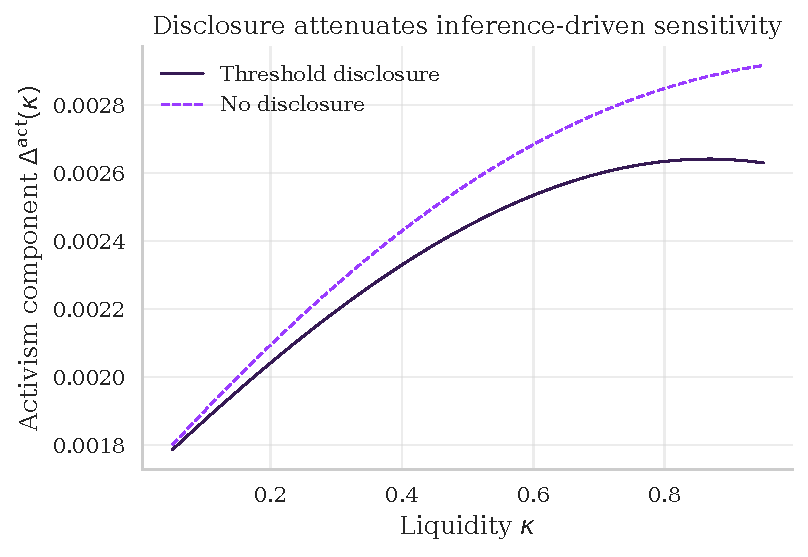
\includegraphics[width=0.72\textwidth]{numerical_output/fig_disclosure.pdf}
\caption{The disclosure-regime comparison in the one-round predecessor model, at fixed cutoffs
($\Omega = 0.037$). The solid line with circle markers prices the blockholder's engagement-driven
premium with the market seeing order flow and the disclosure flag (threshold disclosure,
baseline); the dashed line with square markers prices it from order flow alone (no disclosure,
counterfactual). The two curves cross near $\kappa = 0.73$.
At this baseline the flagged cell is \emph{more} liquidity-sensitive than the pooled one (total
variation ratio $1.064$), so this comparison refutes attenuation in $\kappa$ for the regime margin
at this weight. It is a composition fact, not a window test; the window record is
Table~\ref{tab:window-record}.}
\label{fig:disclosure}
\end{figure}

\subsection{From fixed policies to equilibrium}
\label{sec:ge-results}

Theorem~\ref{thm:T1} holds at fixed policies, and hypothesis (T-7) is exactly what fails once the
cutoff vector is allowed to move with $\kappa$. The next result asks what survives that move. It
carries the region as a \emph{named hypothesis} rather than exhibiting one.

\begin{proposition}[C1: the dominance-and-contraction implication in general equilibrium]
\label{prop:C1}
Assume:
\begin{enumerate}[label=(C-\arabic*),leftmargin=3.2em,itemsep=3pt]
\item the along-the-path contraction of Assumption~\ref{asm:AGE}, $L_{\mathcal R} < 1$, in
  \emph{one fixed norm convention} --- an induced operator norm with its dual pairings; a mismatched
  pairing silently voids the implication;
\item $\mathcal R_r$ relatively open in \emph{both} coordinates, with $\kappa \notin \{0,1\}$;
\item an interior single-branch equilibrium;
\item twice continuous differentiability of $\Dact$ in $(k,\kappa,r)$;
\item a non-vanishing \emph{equilibrium} liquidity derivative --- the equilibrium sensitivity
  $\mathcal S^{GE}$, which is distinguished from the fixed-policy sensitivity $\mathcal S$ of
  Definition~\ref{def:premium};
\item strict dominance $g_r^{PE} > \mathcal B_r^{GE}$ on the region, with $g_r^{PE}$ as in
  \eqref{eq:gPE} and $\mathcal B_r^{GE}$ as in \eqref{eq:BGE};
\item the \emph{threshold} margin $r_\tau$ only: the window coordinate is an integer, and nothing
  local is claimed there.
\end{enumerate}
Then the fixed-policy attenuation sign survives in equilibrium on the region:
\begin{equation}
\label{eq:C1}
\partial_r \mathcal S^{GE} \;\le\; -\eta_r \;<\; 0 .
\end{equation}
The sign-coherence hypothesis --- that the fixed-policy attenuation sign agrees with the equilibrium
sign --- is confirmed unused in \eqref{eq:C1}: its work is one of naming, fixing when that conclusion
may be called a survival of the fixed-policy sign. The sign-constancy clause of
Assumption~\ref{asm:AGE} is likewise unused.
\end{proposition}
\resultstatus{Proved as the dominance-and-contraction implication, with the region carried as a named
hypothesis (online appendix); the region itself is not exhibited, and the node evidence
of Remark~\ref{rem:C1record} is numerical.}

\begin{remark}[Dominance-and-contraction nodes, verified on the numerical grid]
\label{rem:C1record}
Eighteen of eighty grid nodes are pointwise \emph{dominance-and-contraction nodes}. The largest
contiguous block is $T = 5$ at $\tau$-percentiles $\{50,70,90\}$ with
$\kappa \in \{0.65,\,0.75,\,0.85\}$; the slack $\eta_r$ has minimum $0.0595$ and median $0.3467$, and
$L_{\mathcal R} \in [0.264,\,0.501]$ everywhere on the grid. These values come from a numerical
calculation reproduced independently. What these nodes establish is narrow and
worth stating exactly: they verify the two pointwise inequalities $L_{\mathcal R} < 1$ and
$\eta_r > 0$ together with supporting diagnostics. They do \emph{not} verify the full antecedent
(C-1)--(C-7) above, and they do \emph{not} exhibit a named nonempty region; a
dominance-and-contraction node is a pointwise numerical fact, not evidence of a region. A
named-region promotion is a separate step and is not claimed. The earlier aspiration, this result
proved on a named nonempty region and numerical off it, is retired as structurally undeliverable
as worded; what is deliverable is the three objects above: the implication proved with the region as
a hypothesis, the dominance-and-contraction nodes verified on the grid, and a named-region promotion
left open, for which an $\varepsilon$-ball plus integral-control pattern is the template. The
proof also gives the bound $\mathcal B_r^{GE} = O\bigl((1-L_{\mathcal R})^{-3}\bigr)$, so
the dominance-and-contraction nodes are cubically bounded away from $L_{\mathcal R} = 1$.
\end{remark}

\subsection{What is not claimed}
\label{sec:not-claimed}

The results above do not claim: a global window-margin attenuation sign; $\kappa$-invariance of the
filing-day jump $J$; equilibrium uniqueness; a nonempty general-equilibrium region as a theorem;
endogenous filing before the deadline; noisy or partially revealing flagged-round trading;
continuous-time execution; welfare or optimal rule design; that the predecessor model's
non-monotone result for minority gains survives in the two-round model; that the predecessor
calibration at $\Omega \approx 0.037$ is economically meaningful; or any empirical value for the
disclosed share of engagements $\omega_a$: the calibration target has no empirical
anchor in the literature, and the paper does not invent one.

Three questions remain open, in whole or in part, and are recorded as such.
\begin{enumerate}[label=(\arabic*),leftmargin=2.4em,itemsep=3pt]
\item \emph{Whether the two-round pooled cell of Section~\ref{sec:timing} satisfies $\Atau$.}
  Lemma~\ref{lem:L3} shows that the entire remaining bite of the restriction is its support
  condition, exhibits a one-round market that satisfies it and a no-disclosure structure that does
  not, and names the weakest sufficient conditions for the two-round case. Lemma~\ref{lem:L3},
  leg 3 of Lemma~\ref{lem:L4} and Part~(B) of Theorem~\ref{thm:T1} are all conditional on it, which
  makes this the largest single conditionality the results carry.
\item \emph{Whether the existence assumptions can be satisfied for relevant menus, including the
  incentive-compatibility question for a fully separating plan.} Menus satisfying
  Assumption~\ref{asm:A7p} are fully separating on the flagged set, so the remaining burden is
  incentive compatibility, which Proposition~\ref{prop:P1} does not settle. The proposition also
  does not claim that an equilibrium satisfying Assumption~\ref{asm:A8} exists. Nonexistence is
  neither claimed nor shown.
\item \emph{Whether the scoped continuity problem in Assumption~\ref{asm:A6} can be repaired
  constructively.} Remark~\ref{rem:A6record} identifies the cell-edge and collapse-face locus and
  the two constructive routes that could replace the continuity half of the hypothesis; neither
  route is established here.
\end{enumerate}

%==============================================================================
\section{Empirics: motivating facts and the written specification}
\label{sec:empirics}
%==============================================================================

The empirical half of the paper has two layers with different statuses, and the draft keeps them
apart. The motivating facts in Section~\ref{sec:facts} have been run: they are descriptives computed
from the seeded filing sample, with the sample stated exactly and no standard errors claimed. The
specification in Section~\ref{sec:spec} is prospective: it states the variables, windows, samples,
standard errors, placebos, and decision rules before any estimate exists. The timing split is the
specification's default headline; final selection remains pending in
Section~\ref{sec:headline-shell}.

\subsection{Motivating facts: the delay distribution before and after the acceleration}
\label{sec:facts}

The anchor is the February 2024 acceleration: the initial Schedule 13D deadline moved from ten
calendar days to five business days for trigger dates from 2024-02-05 \citep{SEC2023}. The first
question is whether filers moved at all. They did. Drawing a seeded sample of roughly one hundred
fifty initial 13D filings from each of two windows (2023Q2--Q3, the last full pre-rule quarters,
and 2024Q3--Q4, well after the effective date) and measuring the trigger-to-filing delay in
business days with the federal-holiday calendar, the distribution compresses sharply
(Table~\ref{tab:fact1} and Figure~\ref{fig:fact1}).

\begin{table}[H]
\centering
\caption{The trigger-to-filing delay in business days, before and after the February 2024
acceleration. Seeded samples of initial 13D filings drawn from EDGAR, with the trigger date read
from the filing itself and the delay counted in business days on the federal-holiday calendar. Of
the $300$ sampled filings ($150$ in each window), $198$ carry a trigger date that parses: $102$ pre
and $96$ post, which are the parse rates of $0.68$ and $0.64$ against the $150$ drawn per window.
An admissible band of $0$ to $60$ business days then screens out ten of those, $4$ pre (delays of
$129$, $143$, $526$ and $567$ business days) and $6$ post (delays of $62$, $73$, $133$, $262$,
$407$ and $1{,}365$ business days), and the statistics below are computed on the $188$ that remain
($98$ pre, $90$ post). Because the parse rates are below one, every count is a floor. Descriptive
statistics; no standard errors are claimed.}
\label{tab:fact1}
\begin{tabular}{lcccccc}
\toprule
Window & $n$ & Mean & Median & p90 & Share $\le 5$ bd & Share $\le 10$ bd \\
\midrule
Pre (2023Q2--Q3, 10-calendar-day rule)  & 98 & 9.63 & 7.0 & 23.0 & 35.7\% & 80.6\% \\
Post (2024Q3--Q4, 5-business-day rule)  & 90 & 6.40 & 5.0 & 11.1 & 75.6\% & 88.9\% \\
\bottomrule
\end{tabular}
\end{table}

\begin{figure}[H]
\centering
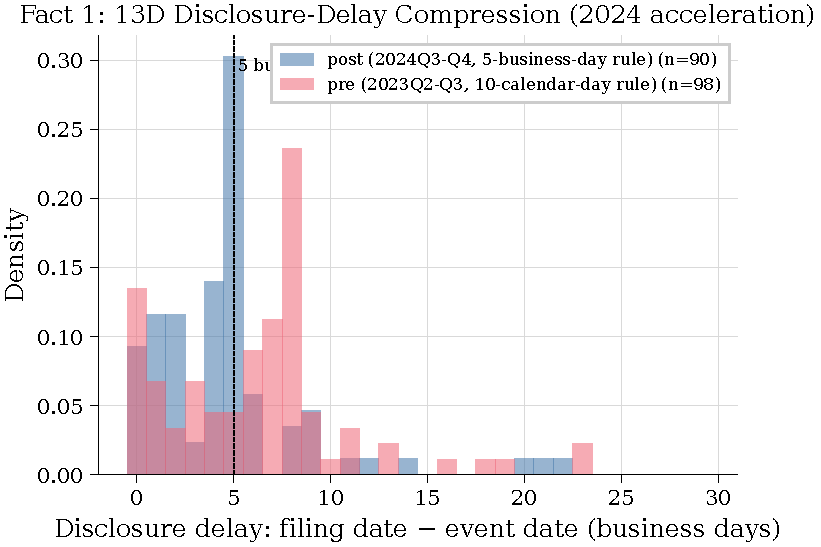
\includegraphics[width=0.72\textwidth]{empirics/output/fact1_delay.pdf}
\caption{The filing-delay distribution, pre (2023Q2--Q3) versus post (2024Q3--Q4) acceleration, in
business days. The mass under the old ten-day regime piles between five and ten business days, with
a long right tail of late filers; under the five-business-day rule the mass concentrates inside the
new deadline. Descriptives from the seeded samples of Table~\ref{tab:fact1}.}
\label{fig:fact1}
\end{figure}

Three readings of the table, each bounded. First, the compression is real and large: the median
delay falls from seven business days to five, and the share of filings inside the new five-day
deadline more than doubles, from 35.7 to 75.6 percent. Second, the pre-rule distribution was not
bimodal. It was already
spread across the old window in the way \citet{BebchukBravJacksonJiang2013} document on filings by
engaging investors: the mass rises into the deadline bucket, where 45.3 percent of their filings sit
at eight to ten business days, with 16.5 percent inside three business days and a tail of 7.1
percent beyond fifteen. The acceleration bit a population that was heterogeneous in exactly the
dimension the rule targets; the design below exploits that heterogeneity as a dose. Third, the numbers agree in kind with the Commission's own
arithmetic: the release expected earlier filing for about 59 percent of timely 13D reports and put
about 29 percent of 2022's initial filings already inside the amended deadline, against our 35.7
percent already inside before the rule. Different samples and different windows, but the same
direction \citep{SEC2023}. The honest caveats travel with the table: the samples are seeded draws,
not the universe; the parse rates are floors; ten filings whose measured delay falls outside a
nought-to-sixty business-day band are screened out and counted in the table note rather than cut
silently; and these are descriptives, with no standard errors, because none are claimed. The delay is counted in business days throughout; counting calendar
days against a business-day rule, as \citet{PolkBuchheitRileyStone2024} do, misclassifies the
48 percent of their sample that piles at their day-ten marker.

\subsection{The written specification for the full empirics}
\label{sec:spec}

This subsection summarises a design fixed before estimation; nothing in it has been run. Every
estimate the December draft will report is specified here or in the underlying document, and the
rule the design imposes on itself is that no specification may change after an estimate is seen, and
that a null is reported with its minimum detectable effect rather than as ``no effect''.

\paragraph{Sample and split.}
The universe is all initial Schedule 13D filings from 2022-01-01 to 2025-12-31, enumerated from
EDGAR quarterly indexes, matched to CRSP. The treatment split is on the \emph{trigger} date, not the
filing date: the deadline attaches to the crossing, so a block crossed on 2024-01-30 and filed on
2024-02-08 belonged to the old regime. Filings that straddle are excluded and counted. The main
pre window is 2022-01-01 through 2023-10-09. The adoption date, 2023-10-10, begins a separately
reported adoption-to-effect stub through 2024-02-04; the stub is not pooled into ``pre''. The
structured-data mandate on 2024-12-18 is a second measurement break, so the main sample ends on
2024-12-17 and 2025 is reported as an extension with its own parse-rate table. The EDGAR
dissemination cut-off moved from 5:30 pm to 10:00 pm ET on the same date the window changed, which
shifts the flagged day by one for part of the post sample; the effective filing date FD$^{*}$ is
constructed to absorb this, and re-running with FD$^{*} \equiv$ FD is a required robustness row. A
full re-fetch and re-parse with the current parser is a stated precondition for any estimate, and
every count in the design is a floor until it has run.

\paragraph{(a) The timing split.}
For every filing, two abnormal returns from a market model estimated over $[\mathrm{TD}-252,
\mathrm{TD}-22]$: the \emph{run-up}, from the trigger to the day before the flag lands, and the
\emph{jump}, on the filing day (a three-day window around the effective filing date). This is
Lemma~\ref{lem:D1}'s identity \eqref{eq:runup-jump} and Lemma~\ref{lem:L2}'s invariance turned into
a regression pair. The partition test (H1) is sign-free: the run-up's liquidity slope should be
non-zero, the jump's zero, and the two different. It is estimated as one
stacked regression with a flagged-half interaction, so the difference carries a standard error;
inference is two-way clustered on subject firm and on calendar month, with a wild cluster bootstrap
on the month dimension and the more conservative of the two reported. The reform test (H2) asks
whether the run-up's liquidity slope changed after February 2024, on a fixed five-trading-day window from
the trigger so the outcome's length does not change mechanically with the rule; both signs are
written out in advance: attenuation (the shorter window moves mass to the $\kappa$-invariant
flagged cell and flattens the composite slope) and amplification (the same informed trading
concentrated into fewer days steepens it). One check can kill the identity: if the jump's
slope moves the same way as the run-up's, there is no partition to write about. Liquidity is a
pre-treatment Amihud-type illiquidity measure, inverted and standardised within quarter, with the
orientation printed in every table note. The run-up \emph{path} from trigger to filing, cut by
liquidity tercile and period, is reported as a figure in the house style, descriptive only; the
benchmark shape is a $0.9$ percent abnormal return on the trigger date and $1.6$ percent on the day
after \citep{PolkBuchheitRileyStone2024}, with the run-up beginning on the trigger date itself
\citep{Zeng2026}.

\paragraph{(b) The bindingness dose.}
The rule binds filers unevenly: those already filing inside five business days cannot be moved by
it. The primary dose is a filer attribute built from pre-period behaviour only and is computed for
filers with at least two pre-period initial 13Ds: the share whose delay exceeded five business days,
in $[0,1]$. For a single-filing filer, a leave-one-out pre-period stratum mean, by filer type,
size tercile and illiquidity tercile, is imputed only in a robustness row and never in the primary
estimate. The dose specification interacts the dose with Post and clusters on filer as well. Its first stage is
mechanical (a fast filer cannot get faster) and is labelled a validity check, not a finding; the
only working-paper estimate of the same first stage is \citet{Trivedi2026}'s compliance share, $+0.348$
with standard error $0.130$, whose own primary outcome, mean lag, is null, and whose sampling
frame is never stated. Because slow filers are plausibly smaller and less liquid, the correlation
between dose and liquidity is reported, and the dose specification is re-run within liquidity
tercile.

\paragraph{(c) Stake at filing.}
The percent of the class printed on the 13D is the empirical counterpart of the model's stake at
filing $B^F$, an object the two-round model produces and the predecessor model could not. The
specification asks whether the stake at filing fell after the acceleration and whether the fall is
ordered by liquidity. One hazard is stated before the estimate because it points the other way: in
the cross-section of delays, \citet{BebchukBravJacksonJiang2013} find the \emph{negative} gradient:
filers who take longer end up with smaller stakes, $0.6$ percentage points per ten days. The
cross-section of delays is therefore never read as a window effect; only the reform is. The historical
days--stake gradient implies a mechanical stake change of roughly $0.12$ percentage points from the
two-day median-delay cut, against the stake leg's minimum detectable effect of $0.85$ percentage
points on the post-re-parse projection, so a detectable
estimate would have to be behavioural rather than arithmetic, and the paper would have to say which.

\paragraph{(d) The bounded null.}
The Commission's own tables cap what the accumulation channel can do. Classifying 2011--2021
non-corporate-action initial 13Ds by how much of the reported stake was already accumulated by the
amended five-business-day deadline: 80 percent of campaigns were unconstrained; 20 percent would
have had some accumulation cut; 3 percent would have had at least a tenth of the stake cut; 1
percent at least a quarter \citep{SEC2023}. If only constrained campaigns can have their bid
outcomes moved by the rule, the aggregate effect on the twelve-month bid hazard is capped by the
constrained share, and the design reports the whole ladder (20, 3 and 1 percentage points)
rather than picking one. The 3-point rung is a judgement about what counts as a materially cut
campaign, and it is stated as such. The bound covers the accumulation channel only; it is not the
aggregate footprint of the rule, and the dollar figures that travel with it in the release are the
Commission's own, and the Commission disclaims them.

\paragraph{(e) The matched difference-in-differences on the bid hazard.}
The control-outcome leg asks whether a bid arrives within twelve months of the trigger, for 13D
targets against \emph{never-13D} firms matched three-to-one on size, illiquidity, industry and
quarter, each control inheriting its treated firm's trigger date as a pseudo-trigger so both are
measured over the identical calendar window. Never-13D rather than 13G controls: 13G filers
disclaim control intent, and selection between the two forms is itself plausibly responsive to the
rule. Bid arrival is coded from tender-offer and merger filings, with a thirty-filing hand audit
done blind. Base rates anchor the power arithmetic: 18.1 percent of campaign targets are acquired
within twelve months against 7.2 percent of matched controls \citep{GreenwoodSchor2009}. The power
arithmetic gives minimum detectable effects of $5.8$ percentage points on today's counts, $4.4$
percentage points for S1 after the re-parse, and $9.9$ percentage points for S2. The latter two use
the optimistic projection $N \approx 4{,}950$, $w \approx 0.394$; they are projections, not estimates.
The MDE exceeds the 3-point ceiling of the bounded null, so the difference-in-differences cannot
separate the accumulation effect from zero even at that ceiling. Only an estimate's excess above
3 percentage points can be attributed to incumbent defence or selection; the first 3 points remain
compatible with accumulation.

\paragraph{(f) Bidder entry by liquidity.}
Within the 13D sample, the bidder-entry leg estimates the liquidity interaction
\begin{equation*}
\mathrm{BID12}_i = \alpha + \delta(\mathrm{LIQ}_i\times\mathrm{Post}_i) + \beta\,\mathrm{LIQ}_i
  + \gamma\,\mathrm{Post}_i + X_i'\theta + \mathrm{FE} + \varepsilon_i .
\end{equation*}
Against the matched never-13D controls it estimates the matched triple difference
\begin{equation*}
\mathrm{BID12}_i = \alpha + \tau(\mathrm{Treat}_i\times\mathrm{Post}_i\times\mathrm{LIQ}_i)
  + \text{all lower-order interactions} + X_i'\theta + \delta_{\mathrm{match}} + \varepsilon_i .
\end{equation*}
The coefficient $\tau$ asks whether the reform's effect on bidder entry differs by liquidity. A
rule-of-thumb power calculation gives projected MDEs of about $8.8$ percentage points for S1 and
$19.8$ percentage points for S2. These are weakly powered projections, and the realised variance
will replace the rule of thumb before an estimate is interpreted.

\paragraph{(g) The referee checklist.}
Control group or bounded null: both, as above. Confounds: ten named ones with a stated handling
each, including the three the literature specifically warns about: the EDGAR cut-off moving on
the same date as the window, calendar-day screens that stop being neutral under a business-day rule,
and the incumbent-defence channel, which runs opposite to accumulation. Rights-plan coverage is
untested: the proposed moderator uses best-effort EDGAR searches for $8$-K Item 3.03 and $8$-A12B;
if coverage is insufficient, the defence channel is retained with its signed-bias fallback. Power:
computed from counts on disk plus stated variance assumptions, with the arithmetic shown; the timing split
detects $1.1$--$2.3$ percentage points per standard deviation of illiquidity after the re-parse,
against a mean pre-rule run-up of $2.8$ percent \citep{Zeng2026}, and anything smaller is reported
as a bounded null. Placebos: 568 holiday-adjusted pseudo-reform dates before the adoption, every
one, plus a pseudo-trigger placebo one quarter before the real crossing and a descriptive 13G
placebo whose deadlines did not change until September 2024. Pre-trends: quarterly liquidity-slope
estimates over the seven pre-adoption quarters, joint $F$-test, and a fixed blocking rule:
a $p$-value below $0.10$ removes causal language from the leg. Parser validation remains incomplete:
the available pipeline output is pre-XML and the full-universe re-parse has not run; both limitations
are reported.

\subsection{Headline shell}
\label{sec:headline-shell}

The headline empirical result is a choice that has not been made, and this subsection is a shell:
it fixes what the headline subsection must contain, lists the candidate headlines with what each
would claim and what would kill each, and marks the choice pending rather than picking one. \\
\textbf{[headline choice pending]}

\paragraph{Candidate A: the partition test as headline.}
Claim: the run-up's liquidity slope is non-zero, the jump's is zero, and the difference is measured
with a standard error: the paper's identity in one regression pair, sign-free and needing no
theory input. What it needs: the re-parsed sample and the stacked specification of (a). What kills
it: a jump slope that moves with liquidity like the run-up's, which would refute the partition
itself and is reported first if it happens. Scope: it is an identity claim, not a reform estimate,
and a referee will ask what the reform did.

\paragraph{Candidate B: the reform's slope change as headline.}
Claim: the run-up's liquidity slope changed after February 2024, in the direction the window record
of Table~\ref{tab:window-record} points (attenuation at every checked node, composition leg
carrying it). What it needs: the same sample, the fixed-length run-up, and a decision on how much
weight to put on a theory direction whose antecedent $\Atau$ is measured to fail at the implemented
calibration, so the design keeps both branches live and pre-specifies what each sign
means. What kills it: a bounded null (the minimum detectable effect is $1.1$--$2.3$ percentage
points on the post-re-parse projection), which is a reportable outcome rather than a failure. Scope: it is the candidate most
directly about the anchor, and the one most exposed to the theory's honest conditionality.

\paragraph{Candidate C: the bounded null as headline.}
Claim: the accumulation channel's aggregate effect on the bid hazard is capped at about three
percentage points by the Commission's own tables, the matched design cannot separately detect even
the ceiling, and that arithmetic, not a point estimate, is the paper's answer to what the
acceleration could do to control outcomes. What it needs: the matched sample and the ladder of
rungs. What kills it: nothing in the data; the risk is presentation, since it reports a ceiling rather
than an effect. Scope: it is the most defensible statement and the least newsy one, and it can be
combined with either A or B as a supporting leg rather than standing alone.

The choice among A, B, and C is mine, and the December draft's headline subsection will be
written into this shell once it is made.

%==============================================================================
\section{Conclusion}
\label{sec:conclusion}
%==============================================================================

The disclosure rule is the market's partition, and this paper takes the identity literally. A stake
threshold and a filing window split the histories that reach a control decision into a flagged cell
and a pooled one; the window is a primitive of the model rather than a rescaling of noise, and the
stake at filing is an object the model produces. On that ground the paper proves what it can and
records where it cannot. Existence is a conditional whose two main hypotheses about the equilibrium
object are measured to fail at the implemented calibration, stated once, in plain words, because
a reader deserves to know exactly what the proposition does and does not cover. The attenuation
theorem separates the rule's two margins honestly: the threshold margin attenuates with no
dominance condition; the window margin attenuates if and only if a weight ratio times an unsigned
composition ratio is at most one. The general-equilibrium survival of the fixed-policy sign is an
implication with the region as a named hypothesis, plus numerical nodes. The numerical layer reads
the same stack against the implemented calibration and reports an attenuation-direction window
record alongside the measured failure of the chord restriction that would close the loop; the
two facts sit in the same section because they are both true.

The empirics rest on the February 2024 acceleration. The established descriptive fact is that filers moved: the
median delay fell from seven business days to five, and the share inside the new deadline more than
doubled. The specification for everything beyond that is written: a timing split that tests the
partition directly, a bindingness dose, a stake-at-filing leg, a bounded null from the
Commission's own tables, a matched
design on the bid hazard whose honest deliverable is already known to be a ceiling, and a
bidder-entry-by-liquidity leg. The
headline choice is recorded as pending.

Three open questions carry the research forward, the same three that
Section~\ref{sec:not-claimed} records: whether any two-round pooled cell satisfies the
chord restriction's support condition, which is the largest single conditionality in the stack;
whether the existence assumptions can be satisfied on a relevant menu, including the
incentive-compatibility question for a fully separating plan; and whether the scoped continuity
problem in Assumption~\ref{asm:A6} can be repaired constructively. Alongside them stands one open
calibration input that is nowhere load-bearing: the disclosed share of engagements $\omega_a$, for which no
dataset in the literature offers an anchor, and which the paper does not invent. Each question is
about the domain of an assumption
this paper states rather than hides, which is where a theory of a legal rule should leave its
unfinished work.


\printbibliography

\end{document}
